\documentclass[12pt,a4paper]{article}

\usepackage[margin=1in]{geometry}
\usepackage[english]{babel}
\usepackage[T1]{fontenc}
\usepackage[utf8]{inputenc}

\usepackage{longtable}
\usepackage{tabularx}
\usepackage{booktabs}
\usepackage{array}
\usepackage{multirow}
\usepackage{graphicx}
\usepackage{enumitem}
\usepackage[parfill]{parskip}
\usepackage[title,titletoc]{appendix}
\usepackage{amsmath}
\usepackage{fnpos}
\usepackage{geometry}
\usepackage{csquotes}
\usepackage{tikz}
\usepackage{pdflscape}

\usetikzlibrary{positioning}
\usetikzlibrary{calc}
 \tikzstyle{main} = [rectangle, rounded corners, minimum height=0.7cm,text centered, draw=black, font=\scriptsize]
 \tikzstyle{process} = [rectangle, minimum height=0.7cm, text centered, draw=black, font=\scriptsize]
 \tikzstyle{note} = [rectangle, text centered, minimum height=1cm]
 \tikzstyle{arrow} = [->,>=stealth,auto,font=\scriptsize,node distance=3cm, main node/.style={circle,draw}]

\usepackage[hyphens]{url}

\usepackage[backend=biber,url=false,style=authoryear,sorting=nyt,bibstyle=numeric]{biblatex}
\addbibresource{chequeBounce.bib}

\usepackage[acronym,nonumberlist,nomain]{glossaries}
\makeglossary
\loadglsentries{acronyms.tex}

\AtBeginEnvironment{quote}{\smaller}
\makeFNbottom
\geometry{margin=1in}
\renewcommand{\baselinestretch}{1.25}
\setlength{\parskip}{1em}
\setlist{nosep}

\newcommand{\floattabu}[1]{
\vspace*{0.2in}
{\footnotesize
#1
}
\vspace*{0.2in}}


\usepackage[hidelinks,breaklinks]{hyperref}
\usepackage{cleveref}

\title{Characterising cheque dishonour cases in India: Causes for delays and policy implications}
\author{Devendra Damle\thanks{Devendra Damle is a researcher at National Institute of Public Finance and Policy.} and Jitender Madaan\thanks{Jitender Madaan is a professor at Indian Institute of Technology, Delhi.} and Karan Gulati\thanks{Karan Gulati is a researcher at the Vidhi Centre for Legal Policy.}\\ and Manish Kumar Singh\thanks{Manish Kumar Singh is a professor at Indian Institute of Technology, Rourkee.} and Nikhil Borwankar\thanks{Nikhil Borwankar is a practicing advocate.}}

\begin{document}
\maketitle

\begin{abstract}
TO DO
\end{abstract}

\newpage
\tableofcontents
\newpage
\printglossaries
\listoftables
\newpage

\section*{Acknowledgements}
The authors would like to thank the DAKSH Centre of Excellence for Law and Technology for their support. The authors are grateful to thank Sandhya PR and Surya Prakash BS (both from DAKSH) for their extensive feedback on the study. The authors would also like to thank Manaswini Rao (Professor of Economics, University of California San Diego) and Pramod Rao (Group General Counsel, ICICI Group) for reviewing the study and their inputs.

\newpage
\section{Introduction}
\label{sec:introduction}
India has a slow judiciary - courts are clogged with large backlogs \autocite{moog1992delays, debroy2008justice, dutta2019modernise}. As of 8th December 2021, over forty-one million cases were pending across district courts \autocite{njdg2021}. It is estimated that judicial delays cost India around 1.5\% of its GDP annually \autocite{dey2016_cost}. Slow judiciaries also have adverse consequences on the structure and efficiency of markets and the quality of life of citizens \autocite{world2004world, chemin2007impact, rao2020institutional}. Therefore, it is hardly surprising that tackling judicial delay has become a top priority for Indian judges and policymakers.

One reason for the large burden on courts is believed to be the large share of \gls{ni} cases.\footnote{In particular, \S~138 of the Negotiable Instruments Act (Dishonour of a cheque for insufficiency, etc., of funds in the account). Act 26 of 1881} While the NI Act contains several provisions that may lead to a dispute, \S~138, in particular, provides that if a cheque (drawn by a person for paying off a debt or a liability) is returned unpaid due to insufficiency of funds or credit, the payer may be imprisoned for up to two years or with a fine up to twice the amount of the cheque, or both. As per the \gls{lci}, they represent 6.5\% and 7.8\% of all institutions and pendency in Indian courts, respectively \autocite{lci2014_arrears}. As per one order of the Supreme Court of India, they reflect more than 15\% of all criminal cases in the District Courts \autocite{sc2020_makwanavstate}. As per another order, they constitute over 30\% of the total pendency in courts.\footcite[Similarly, a study published by the Department of Justice briefly touches on the burden of such cases on the judiciary and posits that they constitute 34\% of pending criminal cases in Maharashtra.][]{sc2020_138, mahadik2018_maharashtra}

Given this increasing volume and persistent mention of \gls{ni} cases as a major cause of judicial delay, \cite{sridhar2017_cheque} examined the behaviour of cheque dishonour cases in India by looking at the DAKSH database of 67,000 cases spread across Indian courts. In most cases, she found that resolution is delayed well beyond the statutorily prescribed timeline of 180 days. Using 50,000 case level data for eight States and two Union Territories, we also estimate the survival probability (using non-parametric Kaplan-Meier estimation) to understand the proportion of unresolved cases within the stipulated time.\footnote{The dataset used for this analysis is documented in section \ref{sec:data-description}.} Figure \ref{fig:stateSurvival} shows the survival probability (case ongoing) for the \gls{ni} cases for different States. As per our estimate, less than 20\% of the cases get disposed of within the prescribed timeline of 180 days. Also, the probability of case completion within 500 days is less than 50\% for most States.

\begin{figure}[!ht]
\centering
\caption{Survival probability of cases across States}\label{fig:stateSurvival}
\footnotesize
\textit{Note:} The X-axis shows the number of days that a case takes from the date of admission until the outcome. The Y-axis shows the probability of the case continuing up to a given number of days.
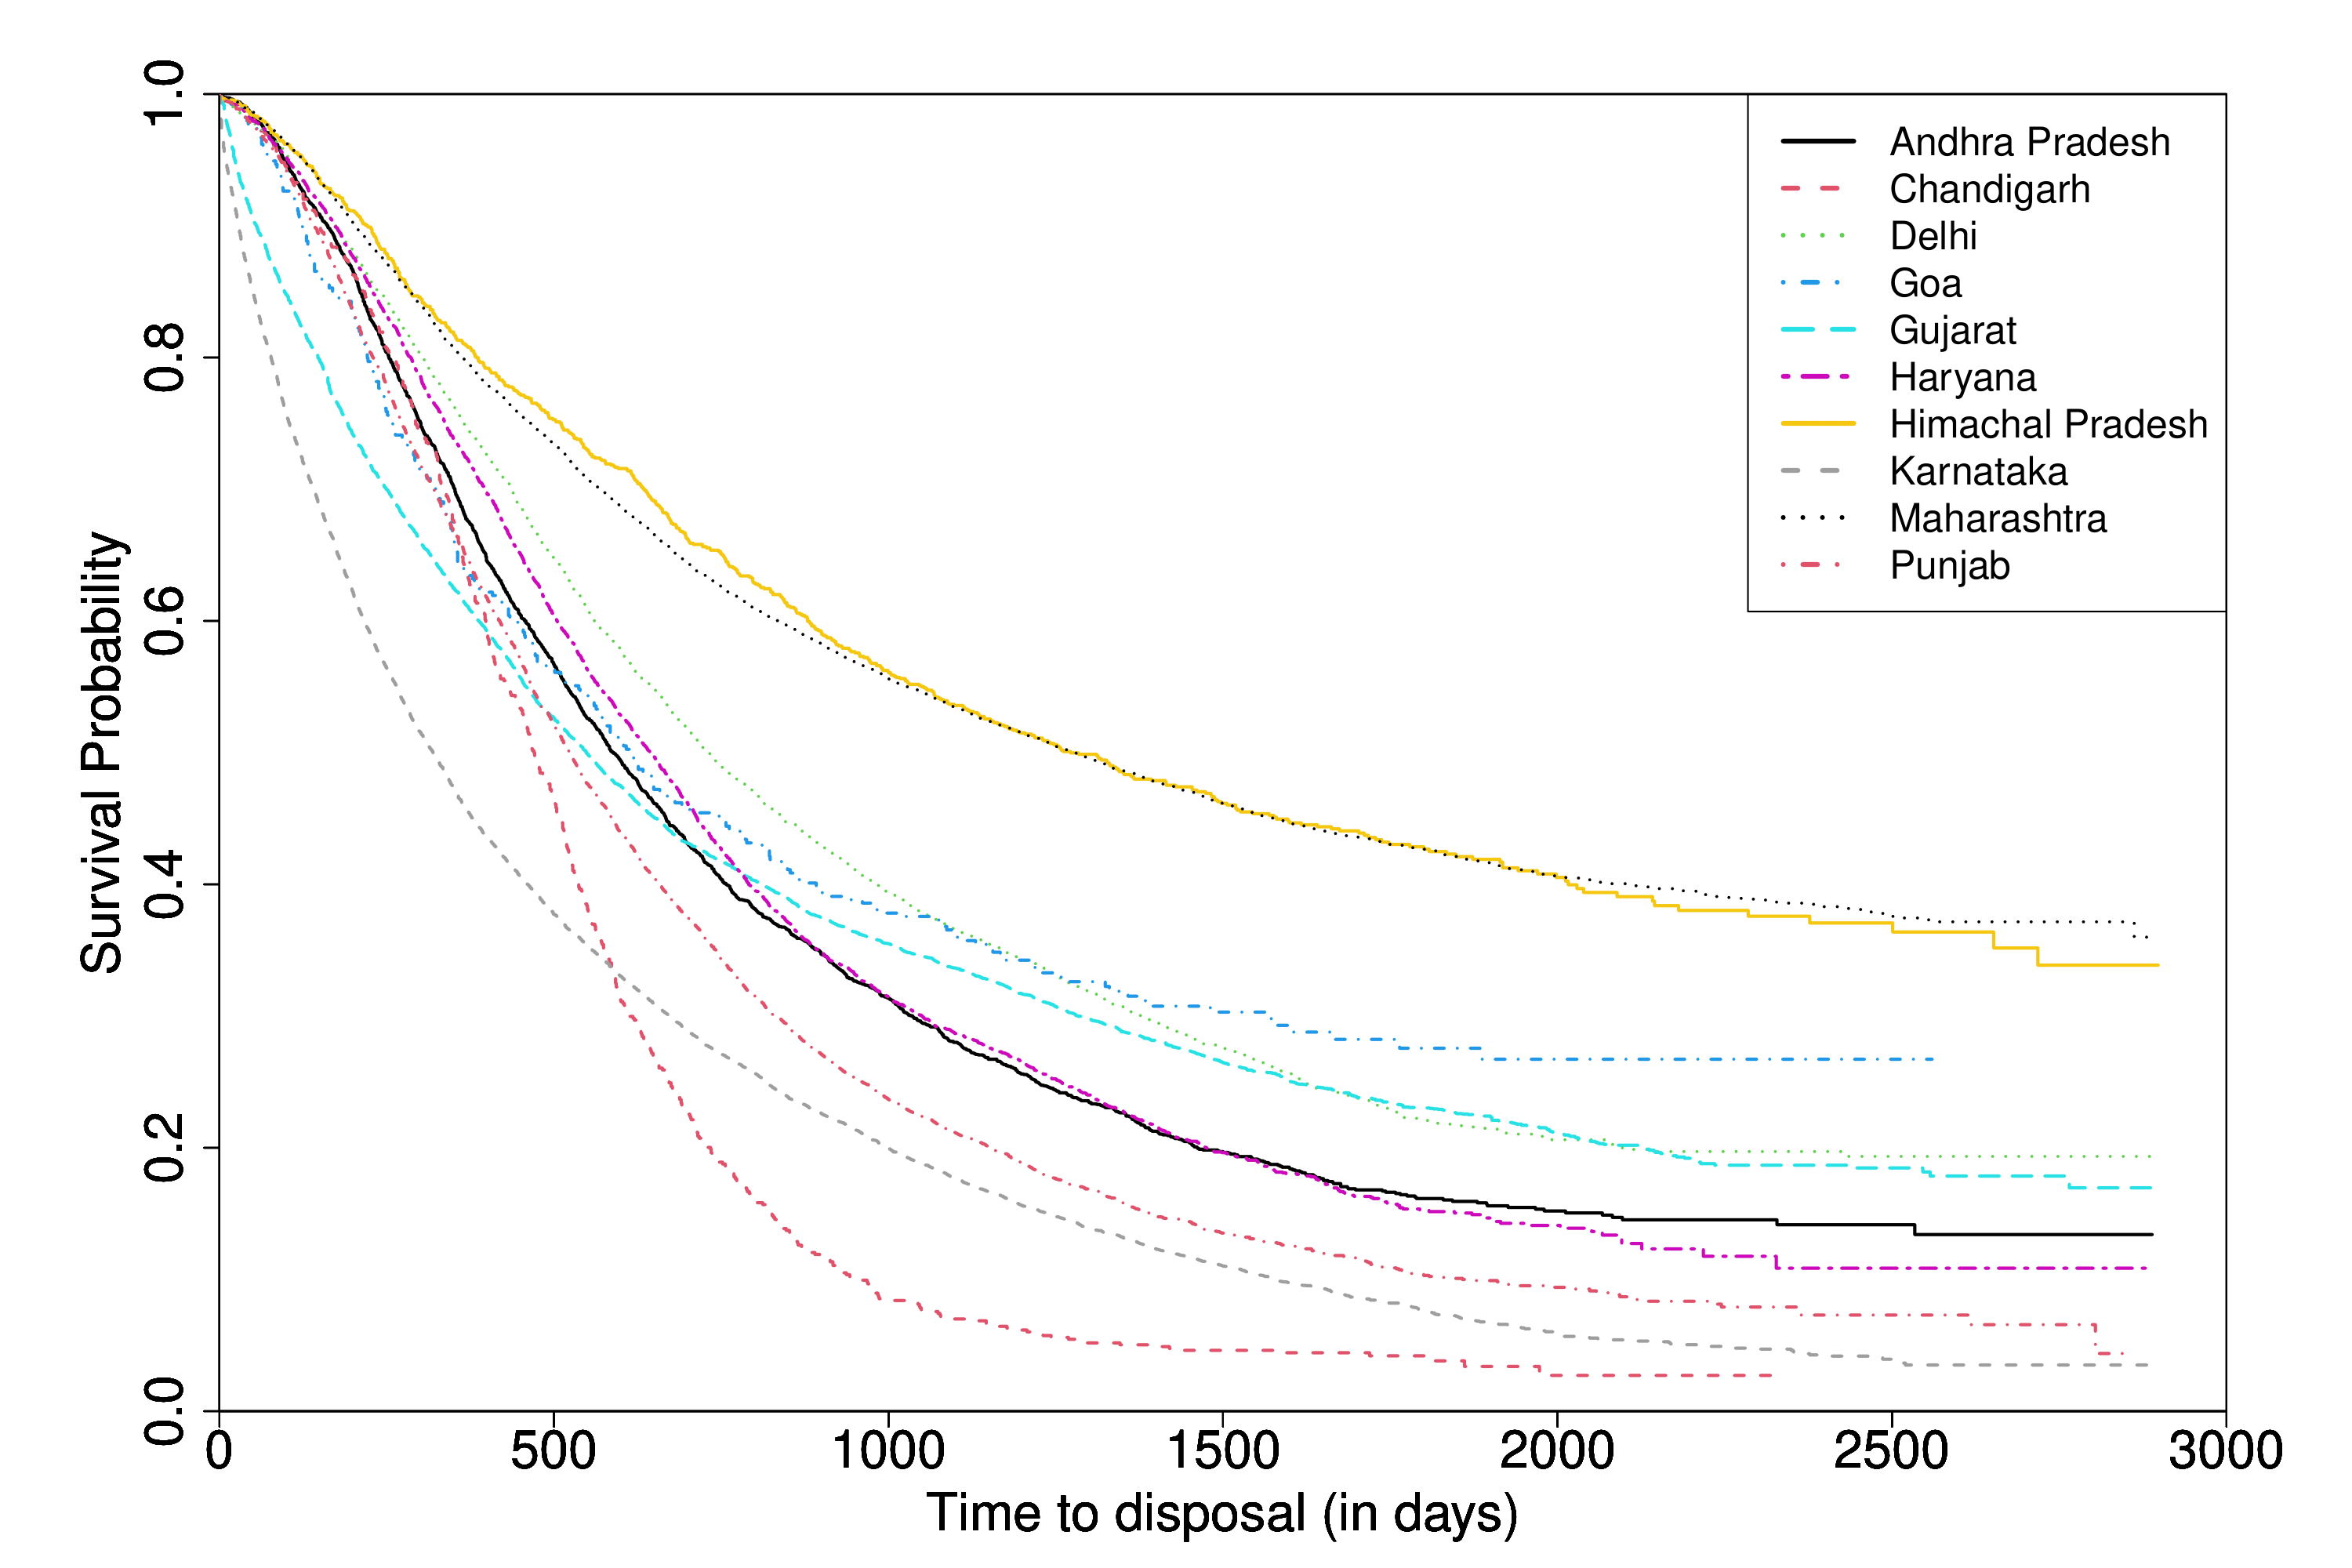
\includegraphics[width=\textwidth]{surv_states-1.png}
\end{figure}

Since cheque dishonour cases are a large burden on the judiciary, various committees, institutions, and government bodies have focused on expediting disposal. For example, the \cite{lci2008_138}, by relying on newspaper reports concerning the proportion of cheque dishonour cases, recommended setting up Fast Track Magisterial Courts (for a detailed discussion, refer to \cite{bhan2015_placing}). The Act was also subject to amendments in 2015 and 2018 to deal with the various procedural matters. Similarly, the Supreme Court has issued directions to lower courts and various financial institutions to take a more pragmatic and realistic approach for the speedy disposal of \gls{ni} cases.

In 2020, the Supreme Court of India took on board a suo-motu case concerning the “expeditious trial of cases under section 138 of the Negotiable Instruments Act 1881” \autocite{sc2020_138}. Among other directions, the court formed a \gls{coe}\footnote{Headed by Hon’ble Mr. Justice RC Chavan, former Judge of the Bombay High Court.} and appointed Amici Curiae\footnote{Mr. Sidharth Luthra (Sr Advocate) and Mr. K Parameshwar (Advocate).} to assist the court, to study processes to expedite the disposal of complaints under \S~138 of the \gls{ni}. In late 2020, the Amici submitted their recommendations. This included (i) increasing the use of pre-and post-summons mediation, (ii) expediting the service of summons to reduce absconsion, (iii) addressing the multiplicity of proceedings, etc. (for additional detail, refer to \cite{amicus2020_submission}).

Given this background, the purpose of this paper is fourfold. First, using case level eCourts data, for the first time in India, we estimate the real judicial caseload due to the \gls{ni}. Second, we estimate the average case disposal time and its variation over time and across States. Third, we build a conceptual framework to establish the link between specific case characteristics and procedural delay. Furthermore, we empirically test our conceptual framework of procedural determinants of case disposal time using regression analysis. In line with \cite{bielen2015}, using case level interim and final orders data, we establish the link between the specific case characteristics and procedural issues while controlling for inherent court and judge characteristics. The empirical literature on the length of court proceedings currently focuses mainly on determinants at the country and court levels, e.g. public budgets for courts, backlogs, number of judges, etc. Some studies also focus on the case level determinants like the number of parties involved, number of pleadings, etc. Given access to the interim and final orders data, we focus on the case characteristics that can be directly targeted using procedural reforms.

Additionally, we examine the role of the Negotiable Instruments (Amendment) Bill, 2015, which was passed by the Parliament in December 2015. The amendment focused on clarifying the jurisdiction-related issues for filing cases for an offence committed under \S~138 of the Negotiable Instruments Act, 1881. It also mandated the centralisation of cases against the same drawer. These reforms were specially drafted to accelerate court proceedings even though no evidence-based insight into the causes of prolonged trials was available. We analyse the effect of the 2015 amendment by comparing the duration of cases handled before and after their implementation using regression analysis. Our research makes it possible to evaluate the effectiveness of these reforms, at least for the States for which we gathered the data.

Our estimates suggest that cheque dishonour cases represent 13.2\% of courts' workload (pending and disposed) in India. This number could be underestimated because, in about 36\% of the cases in the sample, orders were either unavailable or could not be parsed. We also find significant variation in case disposal time across states. Median disposal time varies from as low as 218 days in Karnataka to as high as 547 days in Himachal Pradesh, with a median disposal time of 395 days. We also find that only a fifth of the cases gets disposed of within the prescribed limit of six months.

Controlling for State and year fixed effects, our findings suggest that, all else being equal, cases where the accused fails to appear take an additional 201 days and 7 hearings to dispose of. Similarly, cases run as summons trials take 112 days and 7.4 hearings more than summary trials. Cases with jurisdictional issues take 271 days and 5.5 hearings more to dispose of than cases without these issues. Cases with a multiplicity of proceedings take an additional 168 days and 9.9 hearings to dispose of than those without. Contested cases take fewer days to dispose of than uncontested cases, even though they take more hearings. Our results also indicate that the 2015 amendments have significantly reduced case duration -- reducing the case duration by more than six months.

The rest of this paper is organised as follows: after this introduction, \cref{sec:history} elaborates on the history of cheque dishonour provisions in India and their relation to judicial delays. In \cref{sec:select-case-char}, based on our conversations with practising lawyers, other stakeholders, and the recommendations of the Amici Curiae and the Supreme Court, we figure out the key case characteristics linked to the procedural delay that can be directly targeted by court interventions. \Cref{sec:methodology} describes the methodology, and \cref{sec:results} presents the results thereof. In \cref{sec:2015amend}, we analyse the effectiveness of the 2015 amendments by comparing the duration of cases handled before and after the procedural reforms were implemented. Finally, \cref{sec:conclusion} concludes the paper and presents the way forward.


\section{Cheque dishonour and judicial delays} \label{sec:history}

The \acrlong{ni} was enacted to define the law relating to promissory notes, bills of exchange, and cheques (for an explanation of \S~138, see Appendix \ref{app:understanding}).\footcite{ind1881_niAct} To increase the culture regarding the use of cheques and enhance the credibility of the instrument, the Act was amended in 1988.\footcite{niAmend1988} A new chapter (\S\S~138 to 142) was incorporated for penalties in the event of dishonour of cheques due to insufficient funds in the account of the drawer of the cheque. However, it aimed to include adequate safeguards to prevent harassment of honest drawers. \S~138 provided for the circumstances under a drawer can be penalised for the dishonour of a cheque.

However, by 2001, these provisions were thought not to have had the desired effect.\footcite{stdcomm2001_138niAct} While the punishment was thought to be inadequate, courts could not dispose of cases in a time-bound manner due to the large number of cases pending across the country. Given the large burden on courts, a Working Group was constituted the same year to review \S~138 of the \gls{ni} and make recommendations regarding the changes needed to effectively achieve the purpose of the section.\footcite{wg2001_138} In light of the recommendations of the Working Group, the government decided to bring further amendments to the Act. Among others, the amendments included:

\begin{enumerate}[label=(\alph*)]
 \item increasing the punishment from one year to two years;
 \item providing discretion to the court to waive the period of one month for taking cognisance of a case;
 \item prescribing the procedure for dispensing with preliminary evidence of the complainant;
 \item prescribing the procedure for service of summons via speed post or impanelled private couriers;
 \item providing for summary trials; and
 \item making the offence compoundable.
\end{enumerate}

The amendments aimed at speedy disposal of cheque dishonour cases through their summary trial and making the cases compoundable. The punishment provided under \S~138 also was enhanced from one year to two years. These legislative
reforms aimed to encourage the usage of cheques so that regular business transactions and settlement of liabilities could be ensured. The amendments were considered by the Lok Sabha Standing Committee on Finance, which recommended that given the large burden on courts, the proposed amendments be coupled with the creation of specialised courts for \S~138 cases.\footcite{stdcomm2001_138niAct} However, the subsequent Amending Act did not reference specialised courts.\footcite{niAmend2002} 

\gls{lci} took up the proposal for specialised courts in 2008. According to the Commission, the credibility of the financial sector was facing setbacks due to the large pendency of dishonoured cheque cases. Relying on an array of judgments by the Supreme Court of India concerning speedy trials,\footcite{sc1978_khatoon, sc1981_champalal, sc2005_surinder, sc2008_krishna} the Commission recommended the introduction of fast track courts to address cases concerning dishonour of cheques under \S~138 of the Act. However, it did not comment on the number or expected workload of such courts.\footcite{lci2008_138} The need for additional courts was re-iterated by \gls{lci} in 2009.\footcite{lci2009_reforms}

While \gls{lci} has focused on the need for more courts, the Supreme Court has provided assistance in implementing the amendments. In 2014, noting that the prime reason for the delays in \S~138 case is the absence of the accused, the Court held that the magistrate should adopt a pragmatic and realistic approach such as issuing notices and summons via e-mail or push notification to ensure delivery.\footcite{sc2014_iba} In 2018, the court directed banks to give the details of the e-mail of the accused to the complainant for service through e-mail. The court also directed that: (i) cases must be dealt with summarily, (ii) the evidence of the complainant must be conducted within three months, (iii) an endeavour must be made to conclude the trial within six months, (iv) the trial, as far as practicable, must be held on a day-to-day basis, and (v) High Courts may pass additional localised directions for speedy disposal of cases.\footcite{sc2018_meters}

The Act was also amended in 2015 and 2018 to - clarify the appropriate area of jurisdiction where cheque dishonour cases can be filed,\footcite{niAmend2015} and grant power to courts to grant interim compensation, respectively.\footcite{niAmend2018} In particular, the \citetitle{niAmend2015} 2015 aimed to address the difficulties faced by the payee or lender in filing cases under \S~138 due to a lack of clarity concerning the appropriate forum. It thus inserted specific provisions concerning the jurisdiction for an offence under \S~138, hoping to ensure that a fair trial of cases under \S~138 is conducted keeping in view the parties' interests by clarifying the territorial jurisdiction for trying cases.

On the other hand, the \citetitle{niAmend2018} 2018 aimed to address the delays caused by unscrupulous drawers of dishonoured cheques due to easy filing of appeals and obtaining stay on proceedings. As a result, the payee would have to spend considerable time and resources in court proceedings to realise the value of the cheque. To discourage frivolous and unnecessary litigation, it inserted a new section to provide that a court trying an offence under section 138 may order the drawer of the cheque to pay interim compensation to the complainant, in a summary trial or a summons case, where he pleads not guilty to the accusation made in the complaint; and in any other case, upon framing of charge.

Lastly, in March 2020, the Supreme Court of India took on board a suo-motu case concerning the “expeditious trial of cases under section 138 of the Negotiable Instruments Act 1881”.\footcite{sc2020_138} As mentioned, the court-appointed Amici Curiae to assist in the matter, which presented its preliminary report to the court in October of the same year. The Amici made several suggestions to expedite trial, which among others, includes:

\begin{enumerate}[label=(\alph*)]
 \item Address jurisdictional issues;
 \item Address multiplicity of proceedings; and
 \item Expedite service of summons to reduce absconsion;
 \item Explore setting up specialised courts;
 \item Increase the use of pre- and post-summons mediation;
 \item Mandate presenting of a plausible defence before conversion from summary to summons trial; and
 \item Summon witnesses only when the accused presents a defence.\footcite{amicus2020_submission}
\end{enumerate}

Noticeably, the recommendations of the Amici Curiae were in line with previously accepted reasons for delays in disposal. While considering the recommendations, the Supreme Court recommended the Government and High Courts take necessary action where possible and held that they should be the subject matter of deliberation by the \gls{coe} appointed in the same case.\footnote{Headed by Hon’ble Mr Justice RC Chavan, former Judge of the Bombay High Court.}

\section{Conceptual framework and hypotheses}
\label{sec:select-case-char}

The recommendations of the Amici Curiae and the Supreme Court target several aspects of a \gls{ni} case. They posit that these aspects likely lead to delays. This study examines six areas that are the targets of these interventions, viz. ---

\begin{enumerate}
\item non-appearance by the accused;
\item trials being run as summons trials;
\item reference to mediation;
\item jurisdictional issues;
\item multiplicity of proceedings;
\item setting up additional \gls{ni} courts.
\end{enumerate}

The case characteristics whose impact we have chosen to examine were determined based on two factors: (1) the importance of that characteristic and (2) the feasibility of finding reliable information about it in the eCourts data. Accordingly, we chose to examine the effect of six case characteristics that map onto the six intervention targets mentioned above. The characteristics we chose are as follows:
\begin{enumerate}
\item The accused fails to appear before the court for at least one hearing;
\item The case is converted to a summons trial;
\item The case is referred to mediation;
\item The case has jurisdictional issues and is transferred to another court, as a result;
\item The case contains a multiplicity of proceedings --- either the dishonoured cheque was issued to satisfy multiple transactions, or multiple cheques were dishonoured;
\item The case was contested.
\end{enumerate}

We discuss the salience of each case characteristic and the accompanying hypotheses below.

\subsection{Non-appearance of the accused} 
\label{sec:non-appe-accus}

\textcite{ostrom2000efficiency}, in a study of nine state criminal trial courts in the United States, find that criminal cases where the defendant absconds take 40--90 days longer to dispose than those where the defendant appears in court.\footnote{The authors attribute this to the fact that in such cases, a separate procedure has to be conducted for the judge to issue a bench warrant to produce the accused before the court.} The defendant failing to appear in court is one of the leading causes for failed hearings. Consequently, delays in case disposal in the United Kingdom \autocite{crownProsecutionService2006_magistrateCourtEfficiency}. Similarly, \textcite{llangasinghe1988_fijiJudicialDelays} found that the accused absconding is the most common reason for delays in case disposal in magistrates' courts in Fiji. The Amici Curiae and the Supreme Court's recommendations are premised on the notion that non-appearance of the accused leads to delays. We, therefore, seek to examine whether this holds good for cheque dishonour cases in India. We test the following hypotheses:

\begin{description}
\item[H$_{1a}$]: Cases, where the accused does not appear for one or more hearings, require more days to dispose
\item[H$_{1b}$]: Cases, where the accused does not appear for one or more hearings, require more hearings to dispose
\end{description}

\subsection{Conversion to summons trial}
\label{sec:conv-summ-trial}

We could not find empirical studies on the effectiveness of summary trials in reducing case duration. Procedural law governing summary trials in the United States and United Kingdom are premised on the assumption that summary trials would reduce time delays in case disposal \autocite{miller2003}. At the same time, \textcite{miller2003} argues that regardless of the time-savings that may (or may not) result from summary trials, the discretion it gives to courts violates the principle of the right to a trial by jury. Therefore, bearing in mind the Supreme Court and Amici Curiae's recommendation that, to the extent possible, cases should be conducted as summary trials, and they should be converted to summons trials only in specific situations we test the following hypotheses:

\begin{description}
\item[H$_{2a}$]: Cases converted to summons trials require more days to dispose
\item[H$_{2b}$]: Cases converted to summons trials require more hearings to dispose
\end{description}

\subsection{Cases referred to mediation by the court} \label{sec:furth-exam-cases}

\textcite{buscaglia1997_latinAmericaCourtDelays} find that, in Latin American courts, when judges mandate mediation, it reduces the overall time required to dispose a case.\footnote{They conjecture is that the efficiency gains would result in judges having to dedicate less time to adjudicate such cases.} However, a review of empirical research on the time and cost-effectiveness of court-annexed Alternative Dispute Resolution (ADR), including mediation, by \textcite{wissler2004effectiveness} finds no conclusive relationship between the time required to dispose cases via ADR as compared to going to trial. Some studies reviewed by \textcite{wissler2004effectiveness} find that mediation can increase the duration. Some find that it can decrease the duration, while some find no effect. \textcite{heise2010adr} further finds that participation in ADR does not significantly affect case disposal time. However, cases where the parties choose to settle take less time than ADR. Given the mixed findings on the effect of mediation and the Supreme Court and Amici Curiae's opinion that court-annexed mediation can reduce time to dispose cases, we test the following hypotheses:

\begin{description}
\item[H$_{3a}$]: Cases referred to mediation require more days to dispose
\item[H$_{3b}$]: Cases referred to mediation require more hearings to dispose
\end{description}

\subsection{Jurisdictional issues}

Prima facie, there are four territorial areas involved in a cheque dishonour case - (i) where the issuer ordinarily resides, (ii) where the payee ordinarily resides, (iii) where the cheque was issued, and (iv) where the cheque was presented. 

Prior to 2015, the \gls{ni} only specified circumstances under which complaints concerning cheque dishonour could be filed. It did not specify the territorial jurisdiction of the courts where such a complaint had to be filed. This resulted in individuals filing cases in locations not readily accessible to the opposite party. Thus, cases would have to be transferred to suitable courts for hearing. In 2015, the Act was amended to provide that complaints can only be filed in a court in whose jurisdiction the bank branch of the payee lies.\footcite{niAmend2015} While this addressed the lack of clarity in the court where complaints had to be filed, invariably, cases commenced in territorial jurisdiction where the accused did not ordinarily reside.\footcite{amicus2020_submission}

Such jurisdictional issues, where cases have to be transferred from one court to another, may lead to delays.\footcite{sc2020_138, amicus2020_submission} We thus test the following hypotheses:

\begin{description}
\item[H$_{4a}$]: Cases with jurisdictional issues require more days to dispose
\item[H$_{4b}$]: Cases with jurisdictional issues require more hearings to dispose
\end{description}

\subsection{Multiplicity of proceedings}

\S~219 of the \gls{crpc} provides that when a person is accused of more than one offence of the same kind committed within twelve months, all offences may be tried together, subject to a maximum of three such offences. Similarly, as per \S~220, if a person commits more than one offence in one transaction, she may be charged with all offences and tried at one trial. Experience has shown that a single financial transaction may lead to the dishonour of multiple cheques. However, under the \gls{crpc}, only three offences and, therefore, the dishonour of only three cheques can be tried together. This has resulted in multiple proceedings involving either the same issuer (accused) or the same transaction. Reducing such multiplicity may reduce the burden on courts. We thus test the following hypotheses:

\begin{description}
\item[H$_{5a}$]: Cases involving a multiplicity of proceedings require more days to dispose
\item[H$_{5b}$]: Cases involving a multiplicity of proceedings require more hearings to dispose
\end{description}

\subsection{Contested cases}
\label{sec:contested_cases_meth}
When cases are contested, parties lead evidence before a court and rebut arguments. This is likely to lead to longer proceedings since courts have to come to reasoned decisions based on the proceedings. On the other hand, uncontested cases use minimal court resources, since parties reach a mutually acceptable decision verified by the court. \textcite{ostrom2000efficiency} find that cases that went to trial took 53--158 days longer to dispose than cases where the defendant pleaded guilty.\footnote{The variation in the average delay is between the different jurisdictions studied.} \textcite{buscaglia1997_latinAmericaCourtDelays}, in a study of judicial efficiency in Latin American courts, find that willingness to litigate increases the duration of court cases and results in a greater backlog of cases. \textcite{crownProsecutionService2006_magistrateCourtEfficiency} finds that, in magistrate courts in the United Kingdom, contested cases typically take a greater number of hearings to dispose than uncontested cases. Contested cases take longer to dispose than uncontested cases. The difference between the time it takes the courts to dispose of uncontested cases compared to contested cases can yield insights into how efficient the court is at handling cases that go to trial, compared to cases where the defendant is willing to settle or compound. We thus test the following hypotheses:

\begin{description}
\item[H$_{6a}$]: Contested cases require more days to dispose
\item[H$_{6b}$]: Contested cases require more hearings to dispose
\end{description}

In summary, these characteristics represent six different events that can take place in the course of litigating the case.\footnote{These are not mutually exclusive. One or more of these events can occur in the same case.} We test whether the event's occurrence affects the case duration and the number of hearings required to dispose it. Table \ref{tab:expected} presents a summary of the expected effects of the identified case characteristics. The potential effectiveness of the Supreme Court and Amici Curiae's recommendation of setting up more \gls{ni} courts can be indirectly tested through this characteristic. 

\begin{longtable}{@{}lcc@{}}
\caption{Expected effects of case characteristics}
\label{tab:expected}\\
\toprule
\multicolumn{1}{c}{\multirow{2}{*}{\textbf{Case characteristic}}} & \multicolumn{2}{c}{\textbf{Expected effect}} \\ \cmidrule(l){2-3} 
\multicolumn{1}{c}{} & \textbf{Duration} & \textbf{Hearings} \\ \midrule
Non-appearance of the accused & + & + \\
Conversion to summons trial & + & + \\
Mediation & - & - \\
Jurisdictional issues & + & + \\
Multiplicity of proceedings & + & + \\
Contested cases & + & + \\ \bottomrule
\end{longtable}

%%% Local Variables:
%%% mode: latex
%%% TeX-master: "paper_chequeDishonour"
%%% End:


\section{Methodology}
\label{sec:methodology}
\subsection{Data description}
\label{sec:data-description}
State selection based on an initial sample check of 100,000 cases.
\begin{itemize}
\item Remove States where we were unable to download sample data (this is because of data quality of the e-courts database);
\item Remove States that do not classify any cases as relating to the Negotiable Instruments Act;
\item Remove States where < 2\% of the final orders (as a proportion of total NI cases) are machine readable and in English.
\end{itemize}

Sample description:
\begin{itemize}
\item We attempted to collect a random sample of 5,00,000 cases from
  10 States and Union Territories filed between 2014/01/01 and
  2018/12/31. We were able to successfully get data for 4,68,855
  cases.
\item We removed cases from District and Sessions courts, since we are
  only interested in original matters. After this filter we are left
  with 3,63,762 cases
\item First, we used regular expressions to check whether the ``Act
  Name'' field references the NI Act.
\item Then, we used regular expressions to search for references to
  the NI Act in the texts of the interim orders and final orders,
  where available.
\item Using the aforementioned method, we got a total of 48,191 NI Act
  cases, out of these 10,693 are pending cases and 37,498 are disposed
\end{itemize}

\begin{longtable}{@{}lrrrr@{}}
\caption{Sample description}
\label{tab:sample_desc}\\
\toprule
\textbf{State} & \textbf{NI Act cases} & \textbf{\%NI Act cases} & \textbf{Non-NI Act cases} & \textbf{Total cases}\\* \midrule
\endhead
Andhra Pradesh & 2640 & 12.4 & 18567 & 21207\\
Chandigarh & 731 & 34.9 & 1364 & 2095\\
Delhi & 5211 & 26.1 & 14742 & 19953\\
Goa & 399 & 12.8 & 2713 & 3112\\
Gujarat & 6756 & 12.0 & 49476 & 56232\\
Haryana & 5326 & 13.7 & 33542 & 38868\\
Himachal Pradesh & 1166 & 8.9 & 11948 & 13114\\
Karnataka & 11195 & 12.9 & 75807 & 87002\\
Maharashtra & 8880 & 9.7 & 82673 & 91553\\
Punjab & 5887 & 19.2 & 24739 & 30626\\
\textbf{Total} & \textbf{48191} & \textbf{13.2} & \textbf{315571} & \textbf{363762}\\* \bottomrule
\end{longtable}

\subsection{Approach to analysis}
\label{sec:approach-analysis}

\subsubsection{Text-mining}
\label{sec:text-mining}

\begin{longtable}{@{}lrrrrrr@{}}
\caption{Number of cases in which we were able to identify characteristics of interest}
\label{tab:case_chars}\\
\textbf{State} & \textbf{Non Appearance} & \textbf{Summons Trial} & \textbf{Mediation} & \textbf{Jurisdiction Issue} & \textbf{Multiplicity} & \textbf{Total} \\
\endhead
Andhra Pradesh & 1674 & 814 & 260 & 210 & 124 & 2640 \\
Chandigarh & 701 & 408 & 204 & 278 & 53 & 731 \\
Delhi & 2062 & 1359 & 1026 & 1045 & 208 & 5211 \\
Goa & 381 & 78 & 90 & 33 & 18 & 399 \\
Gujarat & 5125 & 391 & 402 & 3059 & 107 & 6756 \\
Haryana & 5214 & 3376 & 1731 & 2109 & 540 & 5326 \\
Himachal Pradesh & 864 & 351 & 506 & 299 & 33 & 1166 \\
Karnataka & 5850 & 2002 & 1846 & 953 & 410 & 11195 \\
Maharashtra & 5933 & 963 & 2546 & 3831 & 135 & 8880 \\
Punjab & 5821 & 3134 & 2100 & 2281 & 382 & 5887 \\
\textbf{Total} & \textbf{33625} & \textbf{12876} & \textbf{10711} & \textbf{14098} & \textbf{2010} & \textbf{48191}
\end{longtable}

Explain that this is likely an underestimate because orders cannot be parsed in approx 36\% of the cases.

\subsubsection{Regression model specifications}
\label{sec:model-selection}
To examine the impact of case characteristics on case duration, we rely on two different measures: (1) Duration of the case (in days) and (2) Number of hearings required to dispose of. We perform a multivariate analysis: we regress the performance indicators (i.e., duration of the case and the number of hearings required to dispose of the case) on several potential explanatory variables. We also control for State and year fixed effects. For each performance measure, we estimate the following fixed effect regression model:

\begin{equation}\label{eq:fe1}
\begin{split}
Duration_i \ & or \ Number \ of \ hearings_i \\
& = \beta_1 \ D_1(Non-appearance_i) + \beta_2 \ D_2(Jurisdiction \ Issue_i) + \beta_3 \ D_3(Mediation_i) \\
& + \beta_4 \ D_4(Multiplicity_i) + \beta_5 \ D_5(Summons_i) + \beta_6 \ D_6(Contested_i) \\
&  + \alpha_s + Y_t + \epsilon_{ist}
\end{split}
\end{equation}

where $D_1$ is a dummy variable equal to 1 if the accused was not available / out of station/absconding or absent due to other reasons, $D_2$ is a dummy variable equal to 1 if the case refers to jurisdiction issues, $D_3$ is a dummy variable which takes the value 1 if the case was referred for mediation, $D_4$ is a dummy variable equal to 1 if the case suffers from a multiplicity of proceedings, $D_5$ is a dummy variable which takes the value 1 if the case is marked as summons trial, and $D_6$ is a dummy variable equal to 1 if the case was contested. We use the State and year dummies ($\alpha_s$ and $Y_t$ respectively) to control for the macro-economic reforms and environment.


%%% Local Variables:
%%% mode: latex
%%% TeX-master: "paper_chequeDishonour"
%%% End:


%%% Local Variables:
%%% mode: latex
%%% TeX-master: "paper_chequeDishonour"
%%% End:


\section{Results}
\label{sec:results}
Table \ref{tab:summary_results} shows the summary of results.\footnote{Table \ref{tab:duration_reg} in Appendix \ref{sec:impact-case-char} shows the detailed results of the regression model to estimate the effect of case characteristics on the case duration (in days)} The State in which the case is filed has a large and statistically significant effect on the case duration. Controlling for the State-level effects, all but one of the selected case characteristics significantly increase the case duration.

{\footnotesize \begin{longtable}{@{}p{2.5cm}rrrrr}
 \caption{Summary of results}\label{tab:summary_results}\\
 \toprule
 \textbf{Characteristic} & \multicolumn{1}{p{2cm}}{\textbf{Number of cases}} &
 \multicolumn{1}{p{2cm}}{\textbf{As \% of NI Act cases}}
 & \multicolumn{1}{p{2cm}}{\textbf{As \% of total cases}}
 & \multicolumn{1}{p{2cm}}{\textbf{Effect on days to dispose}} &
 \multicolumn{1}{p{2cm}}{\textbf{Effect on hearings to dispose}}
 \\
 \midrule
 Non appearance of the accused & 33625 & 69.8\% & 9.2\% & +213 & +7.0 \\ \midrule
 Conversion to summons trial & 12876 & 26.7\% & 3.5\% & +111 & +7.2 \\ \midrule
 Mediation & 10711 & 22.2\% & 2.9\% & +108 & +3.3 \\ \midrule
 Jurisdictional issues & 14098 & 29.2\% & 3.9\% & +287 & +5.7 \\ \midrule
 Multiplicity of proceedings & 2010 & 4.2\% & 0.6\% & +171 & +10.0 \\ \midrule
 Contested & 8283 & 17.2\% & 2.3\% & --46 & +2.9 \\ \midrule
 Total & 48191 & 100.0\% & 13.2\% & N/A & N/A \\
 \bottomrule
 \\
 \multicolumn{6}{l}{{\footnotesize \emph{Note: `+' sign
  indicates an increase, while `-' sign indicates decrease.}}}\\
\end{longtable}
}

As with the total duration to dispose the cases, the State in which the case is filed has a large and statistically significant effect on the number of hearings.\footnote{Table \ref{tab:hearings_reg} in Appendix \ref{sec:impact-case-char-1} shows the detailed results of the regression model to estimate the effect of case characteristics on the number of hearings required to dispose the case.} Controlling for the State-level effects, all of the selected case characteristics significantly increase the number of hearings required to dispose the case.

The results for each of the case characteristics are discussed in detail below.

\subsection{Non-appearance of accused}
\label{sec:non-appe-accus-1}

Table \ref{tab:nonAppearance_yearWise} shows the number of cases in the sample in which the accused to failed to appear in at least one of the hearings. It appears that this is a very common occurrence, and consistently so, over the entire observation period.

\begin{longtable}[h!]{@{}lrrr@{}}
  \caption{Cases where accused was absent for at least one hearing}\label{tab:nonAppearance_yearWise}\\
\toprule
\multirow{2}{*}{Year} &  \multirow{2}{*}{Total NI Act cases} & \multicolumn{2}{p{4cm}}{Non Appearance}\\
\cmidrule{3-4}
&& Number of cases & Percentage \\
\midrule\endhead
2014 &   6684 &  4302 &  64.4 \\
2015 &   7324 &  5241 &  71.6 \\
2016 &  10634 &  7527 &  70.8 \\
2017 &  12053 &  8628 &  71.6 \\
2018 &  11454 &  7927 &  69.2 \\
\bottomrule
\end{longtable}

We expected cases with incidences of absence by the accused would take more days and more hearings to dispose. The results, shown in Table \ref{tab:summary_results}, indicate that non-appearance of the accused typically adds 213 days to the total case duration. Further, non-appearance of the accused typically adds 7 hearings to the total hearings required to dispose a case. Both these findings are in line with what we expected.

Therefore, any interventions that the courts can make either to ensure the presence of the accused will help to reduce the case durations and number of hearings to dispose. The suggested interventions for this include serving notice of summons through digital media, such as instant messaging, email, and the Supreme Court's automated notice-service software.

Ordinarily, if the accused fails to appear before the court repeatedly, the court issues a bailable warrant to produce them in court. If the accused still fails to appear, the court issues a non-bailable warrant against under Section 70 of the Code of Criminal Procedure (CrPC). This gives the police the power to arrest the accused anytime, and anywhere. The police are also given the authority to forcibly open or break down the doors and walls of the home or the hiding place of the accused. If the accused still fails to appear in court even after the arrest warrants have been issued without bail, the judge can declare the accused to be a ``criminal accused'' under Sections 82, Section 83 of the CrPC. It can then authorise attachment of the property of the accused, and may order the sale of the property to recover the disputed amount.

So another mechanism to reduce delays due to non-appearance of the accused could be to reduce the time taken to conduct these processes. %some commentary on the personal insolvency regime in India?

\subsection{Conversion to summons trial}
\label{sec:conv -summ-trial-1}

Table \ref{tab:summons_yearWise} shows the number of cases in the sample in which the case was converted from a summary trial to a summons trial. The proportion of such cases as a percentage of the total has grown over the observation period.

\begin{longtable}[h!]{@{}lrrr@{}}
  \caption{Cases that were converted to summons trials}\label{tab:summons_yearWise}\\
\toprule
\multirow{2}{*}{Year} &  \multirow{2}{*}{Total NI Act cases} & \multicolumn{2}{p{4cm}}{Summons trial}\\
\cmidrule{3-4}
&& Number of cases & Percentage \\
\midrule\endhead
2014 &   6684 &  1251 &  18.7 \\
2015 &   7324 &  1880 &  25.7 \\
2016 &  10634 &  2814 &  26.5 \\
2017 &  12053 &  3542 &  29.4 \\
2018 &  11454 &  3389 &  29.6 \\
\bottomrule
\end{longtable}

We expected cases converted to summons trial to take more days and more hearings to dispose. The results, shown in Table \ref{tab:summary_results}, indicate that conversion to a summons trial typically adds 111 days to the total case duration. Further, conversion to a summons trial typically adds 7.2 hearings to the total hearings required to dispose a case. Both these findings are in line with what we expected.

The Supreme Court and the Amici Curiae recommend that most cases be tried summarily. If this is implemented by courts, they can expect to reduce the duration of cheque dishonour cases significantly. The mechanism that the Supreme Court proposes is for courts to not convert cases to summons trials unless the accused presents a plausible defence. Further, the court has to record, in writing, its reasons for conducting the case as a summons trial. This recommendation, by itself, may be of limited use, unless an audit mechanism is put in place to assess how often and for what reason cases are converted to summons trials, and whether it was necessary to do so. This will also necessitate the institutionalisation of a mechanism for regular judicial impact assessments.

\subsection{Cases referred to mediation}
\label{sec:mediation}

Table \ref{tab:mediation_yearWise} shows the number of cases in the sample in which the accused to failed to appear in at least one of the hearings. The proportion of such cases is considerable over the entire observation period.

\begin{longtable}[h!]{@{}lrrr@{}}
  \caption{Cases referred to mediation}\label{tab:mediation_yearWise}\\
\toprule
\multirow{2}{*}{Year} &  \multirow{2}{*}{Total NI Act cases} & \multicolumn{2}{p{4cm}}{Mediation}\\
\cmidrule{3-4}
&& Number of cases & Percentage \\
\midrule\endhead
2014 &   6684 &   997 &  14.9 \\
2015 &   7324 &  1521 &  20.8 \\
2016 &  10634 &  2609 &  24.5 \\
2017 &  12053 &  3100 &  25.7 \\
2018 &  11454 &  2484 &  21.7 \\
\bottomrule
\end{longtable}

The results, shown in Table \ref{tab:summary_results}, indicate that a case being referred to mediation typically adds 108 days to the total time required to dispose it. Further, the case being referred to mediation typically adds 3.3 hearings to the number of hearings required to dispose the case. Both these findings run counter to our hypotheses that cases referred to mediation take less time and fewer hearings to dispose. This also means that the recommendation by the Amici Curiae, calling for more cases to be referred to mediation, will not reduce the delays in cheque dishonour cases. In fact, they will have the opposite effect.

Our data show that the mediation process rarely ends in failure as such. So, few cases going back to the court for adjudication due to the parties not reaching a mediated settlement. Table \ref{tab:mediation} summarises the outcomes of cases referred to mediation. We can count all instances where a case is settled, withdrawn or compounded as successful settlement. These constitute 78.6\% of cases referred to mediation. In other words, the mediation process concludes in a successful settlement in a vast majority of the cases. The case gets sent back to the court for adjudication only in 21.4\% of cases. Read with the result on the duration of cases referred to mediation being longer than other cases; this means that the delays result from issues in the mediation process itself, and not (as the literature in other jurisdictions indicates) in whether or not the parties choose to settle.

{\footnotesize \begin{longtable}{@{}clrrr@{}}
\caption{Outcomes of cases referred to mediation}
\label{tab:mediation}\\
\toprule
 \textbf{Disposal type} & \multicolumn{1}{c}{\textbf{Disposal sub-type}} & \multicolumn{1}{c}{\textbf{Total cases}} & \multicolumn{1}{c}{\textbf{Percentage}} & \multicolumn{1}{p{3cm}}{\textbf{Median duration (in days)}} \\
 \midrule
\endhead
\multirow{3}{*}{Dismissed} & other & 478 & 5.46 & 710 \\
 & settlement & 8 & 0.09 & 512 \\
 & withdrawn & 2942 & 33.58 & 491 \\
 \midrule
\multirow{4}{*}{Disposed} & compounded & 459 & 5.24 & 638 \\
 & other & 1395 & 15.92 & 723 \\
 & settlement & 2945 & 33.62 & 527 \\
 & withdrawn & 213 & 2.43 & 462 \\
 \midrule
 Other & other & 320 & 3.65 & 752 \\
 \midrule
 \multicolumn{2}{c}{\textbf{Total}} & \textbf{8760} & \textbf{100.00} & \multicolumn{1}{l}{\textbf{-}} \\
 \bottomrule
 \multicolumn{5}{p{11cm}}{{\footnotesize \emph{Note: The total is less than the total cases referred to mediation owing to the limitations in the data on disposal type and filing/disposal dates.}}}
\end{longtable}}

Precisely identifying issues with the mediation process requires further investigation. However, until these issues are properly identified and understood, courts referring \gls{ni} cases to mediation will likely result in greater delays and pendency.

One caveat that we need to add here is that according to the practicing advocates whom we consulted, the stage at which the case is referred to mediation has a bearing on whether or not mediation will lead to delays. Further the court's reasons (or lack thereof) for delaying the reference to mediation, or delays in scheduling successive hearings may have a confounding effect. However, a deeper analysis of whether courts delay scheduling for legitimate reasons requires an analysis of the order sheet issued by courts for each hearing. This information is, unfortunately, not available on the eCourts platform. To the best of our knowledge this information is not digitised by most courts. Therefore, we cannot analyse this matter any further with the available data.

\subsection{Jurisdictional issues}
\label{sec:jurisd-issu}

Table \ref{tab:jurisdiction_yearWise} shows the number of cases in the sample in which there was a jurisdictional issue. The proportion of such cases as a percentage of the total, though significant, has fallen slightly over the observation period. The increase in cases with jurisdictional issues, in 2016, is likely to be a consequence of the amendment in 2015, which resulted in more cases being transferred to courts that would now have appropriate jurisdiction.

\begin{longtable}[h!]{@{}lrrr@{}}
  \caption{Cases that had jurisdictional issues}\label{tab:jurisdiction_yearWise}\\
\toprule
\multirow{2}{*}{Year} &  \multirow{2}{*}{Total NI Act cases} & \multicolumn{2}{p{4cm}}{Summons trial}\\
\cmidrule{3-4}
&& Number of cases & Percentage \\
\midrule\endhead
2014 &   6684 &  2089 &  31.3 \\
2015 &   7324 &  2229 &  30.4 \\
2016 &  10634 &  3520 &  33.1 \\
2017 &  12053 &  3360 &  27.9 \\
2018 &  11454 &  2900 &  25.3 \\
\bottomrule
\end{longtable}

We expected cases with jurisdictional issues to take more days and more hearings to dispose. The results, shown in Table \ref{tab:summary_results}, indicate that jurisdictional issues typically add 287 days to the total case duration. Further, jurisdictional issues typically add 5.7 hearings to the total hearings required to dispose a case. Both these findings are in line with what we expected. Considering that, on average, 

\subsection{Multiplicity of proceedings}
\label{sec:mult-proc}

Table \ref{tab:mult_yearWise} shows the number of cases in the sample in which there was a multiplicity of proceedings. The proportion of such cases, as a percentage of the total, is small. However, as \Cref{tab:state_multiplicity} shows, the burden caused due to multiplicity varies across States.

\begin{longtable}[h!]{@{}lrrr@{}}
  \caption{Cases with multiplicity of proceedings}\label{tab:mult_yearWise}\\
\toprule
\multirow{2}{*}{Year} &  \multirow{2}{*}{Total NI Act cases} & \multicolumn{2}{p{4cm}}{Multiplicity of proceedings}\\
\cmidrule{3-4}
&& Number of cases & Percentage \\
\midrule\endhead
2014 &   6684 &  259 &   3.9 \\
2015 &   7324 &  382 &   5.2 \\
2016 &  10634 &  544 &   5.1 \\
2017 &  12053 &  515 &   4.3 \\
2018 &  11454 &  310 &   2.7 \\
\bottomrule
\end{longtable}

We expected cases with multiplicity of proceedings to take more days and more hearings to dispose. The results, shown in Table \ref{tab:summary_results}, indicate that multiplicity of proceedings typically adds 171 days to the total case duration. Further, multiplicity of proceedings typically adds 10 hearings to the total hearings required to dispose a case. Both these findings are in line with what we expected.

This may be due to the excess coordination required on the part of the judiciary. To address this challenge, \citetitle{sc2020_138}, the Amici Curiae appointed by the Supreme Court recommended that:

\begin{enumerate}
 \item The Union Government bring a legislative amendment to address the multiplicity of proceedings where cheques have been issued for one purpose. However, multiple complaints, summons and trials have to be undertaken. 
 \item The Supreme Court issue directions to High Courts to amend their Criminal Rules of Practice (by whatever name called) to ensure that complaints arising out of the same transaction, but resulting in dishonour of multiple cheques be clubbed together and a common process evolved for joint trial.\footcite{amicus2020_submission}
\end{enumerate}

The Court accepted both these recommendations.\footcite{sc2020_138}

\begin{longtable}[h!]{@{}lrrr@{}}
  \caption{Multiplicity of proceedings by state}\label{tab:state_multiplicity}\\
\toprule
\multirow{2}{*}{State} &  \multirow{2}{*}{Total NI Act cases} & \multicolumn{2}{p{4cm}}{Cases with multiplicity of proceedings} \\
        &        & Number & Percentage \\
\midrule
\endhead
Andhra Pradesh   &   2638 &  124 &   4.7 \\
Chandigarh       &    731 &   53 &   7.3 \\
Delhi            &   5202 &  208 &   4.0 \\
Goa              &    399 &   18 &   4.5 \\
Gujarat          &   6752 &  107 &   1.6 \\
Haryana          &   5319 &  540 &  10.2 \\
Himachal Pradesh &   1164 &   33 &   2.8 \\
Karnataka        &  11184 &  410 &   3.7 \\
Maharashtra      &   8875 &  135 &   1.5 \\
Punjab           &   5885 &  382 &   6.5 \\
\bottomrule
\end{longtable}

While on average, 4.2\% of the cases in our sample include a multiplicity of proceedings, this is as high as 10.2\% in Haryana. Notably, the three States and Union Territories with the highest proportion of such proceedings, i.e., Haryana, Punjab, and Chandigarh, all come under one High Court -- the High Court of Punjab and Haryana at Chandigarh. Thus, bringing an amendment to the \gls{crpc} may not be an appropriate use of resources. Instead, in line with the second recommendation by the Amici, there is a need for targeted and context-specific intervention by concerned High Courts.

\subsection{Contested cases}
\label{sec:contested-cases}

Table \ref{tab:mult_yearWise} shows the number of cases in the sample which were contested by the accused. The proportion of such cases, is significant, but appears to have declined over the years. % any reason for this?

\begin{longtable}[h!]{@{}lrrr@{}}
  \caption{Year-wise contested cases}\label{tab:cont_yearWise}\\
\toprule
\multirow{2}{*}{Year} &  \multirow{2}{*}{Total NI Act cases} & \multicolumn{2}{p{4cm}}{Contested cases}\\
\cmidrule{3-4}
&& Number of cases & Percentage \\
\midrule\endhead
2014 &   6684 &  2171 &  32.5 \\
2015 &   7324 &  1944 &  26.5 \\
2016 &  10634 &  1822 &  17.1 \\
2017 &  12053 &  1478 &  12.3 \\
2018 &  11454 &   868 &   7.6 \\
\bottomrule
\end{longtable}

We expected contested cases to take more days and more hearings to dispose than uncontested cases. The results, shown in Table \ref{tab:summary_results}, indicate that contested cases typically take 3 hearings more but 46 days less to dispose than uncontested cases. While the finding on the effect on number of hearings was as we expected, the latter finding regarding the effect on overall duration runs counter to our hypothesis.

In 1925, the Civil Justice Committee noted that there is a temptation to hold back the heavier \textit{contested} suits and devote attention to the lighter ones.\footcite{cg1925_civiljustice} Close to a hundred years later, this conjecture may not hold true for cases under the \gls{ni}. The results imply that courts efficiently dispose cases when both parties participate in the proceedings by scheduling successive hearings in a shorter time than when the matter is uncontested.

While courts may not be able to reduce the number of hearings required to dispose of a contested case, prioritisation and scheduling with minimal delays reflects a positive framework to ensure expeditious trial. However, the proportion of contested cases reduced from 2014 and 2018. Uncontested cases, that form the majority, require less intervention by courts. They are listed after larger gaps. This may be due to parties needing more time to reach a mutually acceptable decision or courts prioritising contested cases. Either case suggests there may be some scope for improving the scheduling mechanism for uncontested cases.

\subsection{Potential impact on case-loads} \label{sec:impact-case-loads}

The delays resulting from the respective characteristics affect a significant proportion of \gls{ni} cases. Since \gls{ni} cases constitute 13.2\% of courts' workload, these delays are bound to contribute to the overall delays in courts. They affect the overall pendency in the judiciary. 

For example, if the problem of accused persons not appearing before the court is addressed, all else being equal, the total duration of over 9\% of cases would reduce by 213 days, and courts will have to allocate 7 fewer hearings per case. Similarly, if jurisdictional issues are addressed, the total duration of close to 4\% of cases would reduce by 287 days, and courts will have to allocate 6 fewer hearings per case.

As per the \gls{njdg}, as of January 2022, there were 3,57,72,846 total original pending cases in subordinate courts in India. Assuming the proportions and ratios of our analysis and results hold good for the country as a whole, 13.2\% of these cases would relate to the \gls{ni}, which would amount to 47,39,902 cases. To put the numbers in the table into context, ensuring the presence of the accused can lead to reducing 2,32,58,415 hearings across courts in the country.\footnote{This assumes the proportion of the distribution of case characteristics holds good for the country as a whole.} Similarly, if all \gls{ni} cases are disposed summarily, courts across the country can avoid 90,86,676 hearings. Further, if none of the cases were to have jurisdictional, 78,48,857 hearings could be avoided overall. While the Supreme Court has provides clarity on the procedure to be followed when the accused does not ordinarily reside within a court's jurisdiction, there is a need for further analysis on how to reduce such cases in the first place, since parties need not ordinarily reside and have bank accounts within the jurisdiction of the same court.

In the same vein, referring \gls{ni} cases to mediation could be adding 34,40,884 hearings to the courts across the country. All these hearings can be avoided if these cases were instead tried and disposed by the court itself. This is significant and highlights why it is necessary to support policy decisions with robust empirical studies.


%Add text about fixed effects and pending cases
%write email

%%% Local Variables:
%%% mode: latex
%%% TeX-master: "paper_chequeDishonour"
%%% End:

\section{Conclusion}
\label{sec:conclusion}
The Amici Curiae and Supreme Court has given the following recommendations to reduce delays and pendency of cheque-dishonour cases:
\begin{enumerate}
\item Increase use pre- and post-summons mediation
\item Expedite service of summons to reduce absconsion
\item Mandate plausible defence before conversion from summary to summons trial
\item Summon witnesses only when the accused presents a defence
\item High Courts should prepare schemes to dispose cases pending for 2-4, 4-6, 6+ years
\item Address multiplicity of proceedings
\item Magistrate should record reasons for conversion of summary to summons trial
\item Explore setting up specialised courts
\item Judicially settle the position of \S~202 CrPC
\item Jurisdictional issues
\end{enumerate}

We have been able to test the likely effect of 5 of the targets of these interventions viz --- trials being run as summons trials, non-appearance by the accused, jurisdictional issues, reference to mediation, and multiplicity of proceedings. We find that most of the intended targets of the Amici Curiae's and Supreme Court's proposals do affect the duration of \gls{ni} cases. So any interventions that can reduce the proportion of cases being converted into summons trials, prevent cases from being filed in the wrong jurisdiction, ensure the presence of the accused, and reduce the multiplicity of proceedings will reduce delays in these cases and will also reduce the number of hearings required to dispose them.

However, we find that cases referred to mediation take significantly longer to dispose. We find that referring more \gls{ni} cases to mediation can in fact increase delays and burden courts even more. Further, there appear to be issues with the mediation process itself, because not many cases return to the courts for adjudication due to the mediation failing.

At the same time, we find that contested cases take fewer days to dispose even though they require more hearings. This indicates that judges might be more efficient at resolving these cases than mediation forums. As a corollary, increasing the number of special \gls{ni} courts might have the intended effect of increasing disposal rates and reducing pendency.

Our research attempts to quantify the effects of different characteristics of \gls{ni} cases on the duration. We rely on texts of judgments and orders for much of this analysis. This approach can be improved upon courts institute systems to produce more granular data on cases. One gap in our analysis, for example, is that we cannot reliably identify why the cheque in question was issued. Further, where orders are not available, our ability to identify the characteristics of interest are limited. That is also one of the reasons we had to omit many of the states from our analysis.

Policy-making and administration are research-dependent processes. Better research requires better data. Therefore, courts should record better data about case characteristics and case flow. This will enable researchers and courts alike to better identify bottlenecks in existing processes and problematic provisions in laws. Courts, in turn, can use these analyses to improve procedures and administration and ensure better justice delivery.

%%% Local Variables:
%%% mode: latex
%%% TeX-master: "paper_chequeDishonour"
%%% End:

\newpage
\begin{appendices}
\section{Understanding \S~138 of the Negotiable Instruments Act} \label{app:understanding}

As per \S~138 of the Negotiable Instruments Act, 1881, if a cheque (drawn by a person for paying off a debt or a liability) is returned unpaid due to insufficiency of funds or credit, the payer may be imprisoned for up to two years or with a fine up to twice the amount of the cheque, or both.\footcite[A \textit{cheque} is defined as per \S~6 of the NI Act. It is a bill of exchange drawn on a specified banker and not expressed to be payable otherwise than on-demand. It includes the electronic image of a truncated cheque and a cheque in electronic form. Once a cheque has been signed and issued in favour of the holder of the cheque, there is a statutory presumption \S~139 of NI Act that the cheque is issued in discharge of a legally enforceable debt or liability. However, said presumption is a rebuttable one. The issuer of the cheque can rebut that presumption by adducing credible evidence that the cheque was issued for some other purpose like security for a loan.][]{sc2018_murugun} However, this is only the case when: (i) the payee presents the cheque within six months of its issuance, (ii) demand for the payment within thirty days of the return of the cheque by the bank, and (iii) the payer fails to pay within fifteen days of the receipt of such notice. The cause of action arises after these fifteen days. The payee subsequently has one month to file a complaint before the appropriate court.

An offence within the contemplation of \S~138 is complete with the dishonour of the cheque, but taking cognisance of the same by any court is forbidden so long as the complainant does not have the cause of action to file a complaint.\footcite{sc2014_dashrath} This is because the legislature has considered it appropriate to allow the drawer of a dishonoured cheque to pay up the amount before permitting her prosecution. The accused has a right to pay the money within fifteen days from the date of the service of notice, and only when she fails to pay is it open for the complainant to file a complaint. Thus, in \citetitle{sc2002_shakti}, where a complaint failed to mention that notice had been served, the same was not maintainable.\footcite{sc2002_shakti}

A complainant may approach the concerned court within one month of the time provided to the payer to satisfy his debt or liability. After an amendment in 2015, the Act has been modified to prescribe that the territorial jurisdiction for filing of a cheque dishonour complaint shall be restricted to the court within whose territorial jurisdiction the offence is committed, i.e., which is the location where the cheque is dishonoured or returned unpaid by the bank on which it is drawn. Place of issuance or delivery of the statutory notice or where the complainant chooses to present the cheque for encashment by his bank is relevant for determining territorial jurisdiction for filing cheque dishonour complaints.

Once a complaint is led in court, the court takes cognisance and issues the process for producing the accused. If the accused fails to appear, the court may issue a suitable warrant to ensure the same. As per \S~143 of the Act, cases are meant to be tried summarily. However, if the court believes that the nature of the matter is such that a sentence of imprisonment for a term exceeding one year may have to be passed or that it is, for any other reason, undesirable to try the case summarily, it may record such an order and hear the cases as a summons trial.\footnote{In case of a summary trial, if the accused pleads not guilty, the magistrate may record the substance of the evidence and deliver a judgment. However, in a summons trial, the proceeding is as any ordinary matter followed by a judgment.}

Notably, the Supreme Court has observed that for the offence \S~138, the compensatory aspect of the remedy should be prioritised over the punitive aspect.\footcite{sc2010_damodar} Waiver of imprisonment instead of payment of additional compensation is permissible under exceptional circumstances.\footcite{sc2018_priyanka} The court may close proceedings if the accused deposits the amount assessed by it regarding the cheque amount, interest/costs, etc., within the stipulated period. Compounding at the initial stage and even at a later stage is acceptable.\footcite{sc2018_meters} 

For brevity, \cref{fig:proceeding_138} demonstrates the course of a proceeding in the case of a cheque dishonour.

\begin{figure}[ht]
\caption{Proceeding \S~138 of the Negotiable Instruments Act}
\label{fig:proceeding_138}
\vspace*{0.5cm}
\centering 
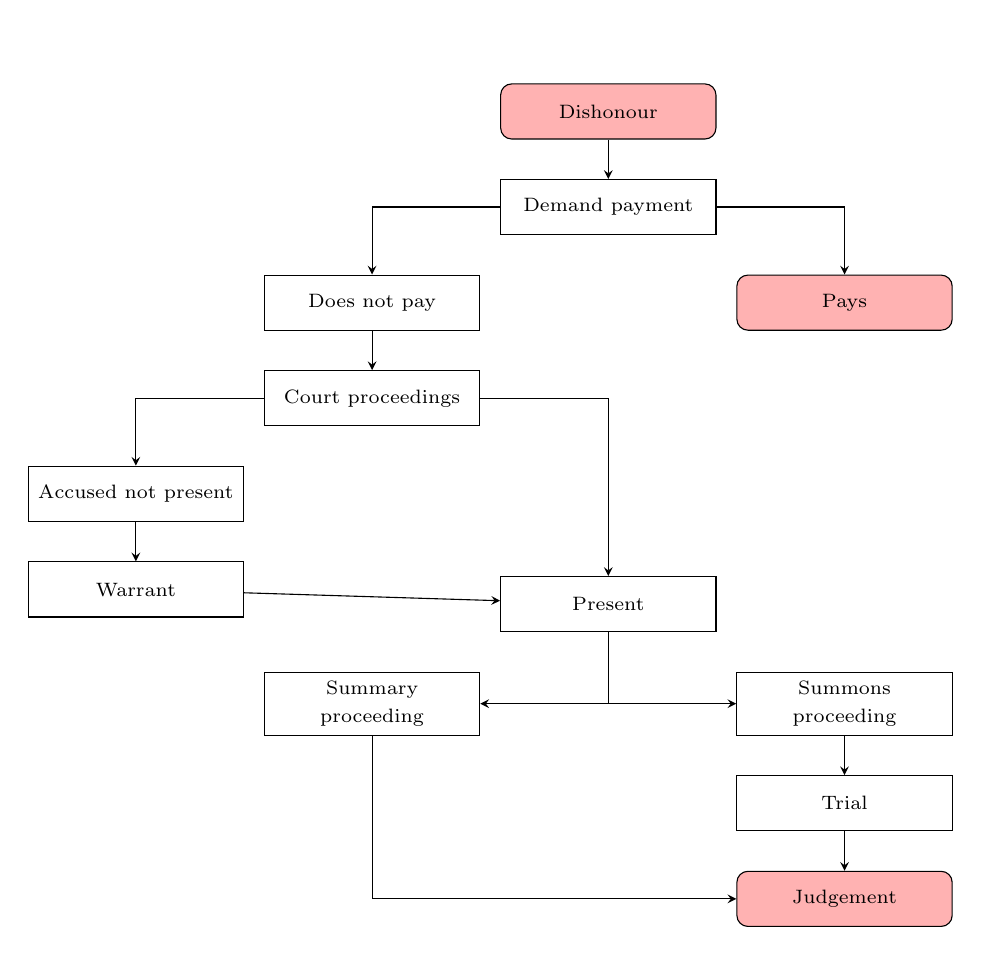
\begin{tikzpicture}[node distance= 1cm, text width=2.5cm]
\node (in0) [note] {};
\node (in1) [main, fill=red!30, below = 0.5cm of in0, yshift = 0.8cm] {Dishonour};
\node (in2) [process, below = 0.5cm of in1] {Demand payment};
\node (in3) [process, below = 0.5cm of in2, xshift = -3cm] {Does not pay};
\node (in4) [main, fill=red!30, below = 0.5cm of in2, xshift = 3cm] {Pays};
\node (in5) [process, below = 0.5cm of in3]{Court proceedings};
\node (in6) [process, below = 0.5cm of in5, xshift = -3cm] {Accused not present};
\node (in7) [process, below = 0.5cm of in6] {Warrant};
\node (in8) [process, below = 1.9cm of in5, xshift = 3cm] {Present};
\node (in9) [process, below = 0.5cm of in8, xshift = -3cm] {Summary proceeding};
\node (in10) [process, below = 0.5cm of in8, xshift = 3cm] {Summons proceeding};
\node (in11) [process, below = 0.5cm of in10] {Trial};
\node (in12) [main, fill=red!30, below = 0.5cm of in11] {Judgement};

\draw [arrow] (in1) -- (in2);
\draw [arrow] (in2) -| (in3);
\draw [arrow] (in2) -| (in4);
\draw [arrow] (in3) -- (in5);
\draw [arrow] (in5) -| (in6);
\draw [arrow] (in5) -| (in8);
\draw [arrow] (in6) -- (in7);
\draw [arrow] (in7) -- (in8);
\draw [arrow] (in8) |- (in9);
\draw [arrow] (in8) |- (in10);
\draw [arrow] (in10) -- (in11);
\draw [arrow] (in11) -- (in12);
\draw [arrow] (in9) |- (in12);

\end{tikzpicture}
\end{figure}

\pagebreak

\section{Criteria for sample selection} \label{sec:sample_selection}

\begin{longtable}{p{0.32\textwidth}p{0.6\textwidth}}
\label{tab:sample_selection}
\\
\toprule
\multicolumn{2}{c}{\textbf{States Excluded}} \\ \midrule
\multicolumn{1}{c|}{\textbf{Criteria}} & \multicolumn{1}{c}{\textbf{States}} \\ \midrule
\multicolumn{1}{p{0.32\textwidth}|}{Unable to download sample data} & \\ \midrule
\multicolumn{1}{p{0.32\textwidth}|}{No cases related to \gls{ni}} & \\ \midrule
\multicolumn{1}{p{0.32\textwidth}|}{\textless 2\% of the final orders are machine-readable and in English} & \\ \midrule
\multicolumn{2}{c}{\textbf{Final Sample}} \\ \midrule
 \multicolumn{2}{p{0.92\textwidth}}{\textit{Andhra Pradesh, Chandigarh, Delhi, Goa, Gujarat, Haryana, Himachal Pradesh, Karnataka, Maharashtra, and Punjab.}} \\ \bottomrule
\end{longtable}

\pagebreak

% \section{Regression results} \label{sec:regression-results-1}

% In the tables below, the rows with the prefix C(stateName) are the State dummies, and rows with the C(year) prefix are the year dummies. \emph{NonAppearance} refers to the accused not appearing in court. \emph{Summons} refers to the case being tried as a summons trial. \emph{Mediation} refers to the case being referred to mediation. \emph{Jurisdiction} refers to the case having some issue with jurisdiction. \emph{Multiplicity} refers to the case either involving multiple cheques or the dishonoured cheque being issued in respect of multiple transactions. \emph{Contested} refers to the case being contested.

% \subsection{Impact of case characteristics on case duration (in days)}
% \label{sec:impact-case-char}
% {\footnotesize
%  \begin{longtable}{@{}lrrrrrr@{}}
% \label{tab:duration_reg}\\
% \toprule
% variable & coeff & std err & t & P>|t| & [0.25 & 0.95] \\\midrule
% \endhead
% Intercept & 407.2465 & 10.065 & 40.462 & 0.000 & 387.519 & 426.974 \\
% C(stateName)[T.Chandigarh] & -266.5441 & 16.731 & -15.931 & 0.000 & -299.337 & -233.751 \\
% C(stateName)[T.Delhi] & 98.8085 & 10.513 & 9.399 & 0.000 & 78.204 & 119.413 \\
% C(stateName)[T.Goa] & -131.1721 & 24.274 & -5.404 & 0.000 & -178.750 & -83.594 \\
% C(stateName)[T.Gujarat] & -161.1733 & 10.013 & -16.097 & 0.000 & -180.799 & -141.548 \\
% C(stateName)[T.Haryana] & -235.2128 & 10.458 & -22.492 & 0.000 & -255.710 & -214.715 \\
% C(stateName)[T.Himachal Pradesh] & 3.8897 & 16.965 & 0.229 & 0.819 & -29.362 & 37.141 \\
% C(stateName)[T.Karnataka] & -121.5457 & 9.110 & -13.342 & 0.000 & -139.402 & -103.690 \\
% C(stateName)[T.Maharashtra] & -10.1451 & 10.067 & -1.008 & 0.314 & -29.876 & 9.586 \\
% C(stateName)[T.Punjab] & -253.8969 & 10.164 & -24.980 & 0.000 & -273.819 & -233.975 \\
% C(year)[T.2015] & 25.6553 & 6.816 & 3.764 & 0.000 & 12.295 & 39.015 \\
% C(year)[T.2016] & 9.7630 & 6.561 & 1.488 & 0.137 & -3.097 & 22.623 \\
% C(year)[T.2017] & -100.5308 & 6.510 & -15.442 & 0.000 & -113.291 & -87.770 \\
% C(year)[T.2018] & -192.9984 & 6.816 & -28.315 & 0.000 & -206.358 & -179.638 \\
% NonAppearance & 213.3056 & 4.855 & 43.932 & 0.000 & 203.789 & 222.822 \\
% Summons & 111.5809 & 5.141 & 21.704 & 0.000 & 101.504 & 121.658 \\
% Mediation & 108.0148 & 4.957 & 21.792 & 0.000 & 98.300 & 117.730 \\
% Jurisdiction & 286.8096 & 4.922 & 58.270 & 0.000 & 277.162 & 296.457 \\
% Multiplicity & 171.0771 & 9.938 & 17.215 & 0.000 & 151.599 & 190.555 \\
% Contested & -46.5545 & 5.244 & -8.877 & 0.000 & -56.834 & -36.275\\
% \bottomrule
% No. Observations & 37175 & & & & &\\
% R-squared & 0.258 & & & & & \\
% Adj. R-squared& 0.258& & & & & \\
% Df Residuals& 37155 & & & & &\\
% F-statistic & 680.7 & & & & & \\
% Log-Likelihood & -2.7359e+05 & & & & & \\
% \bottomrule
% \end{longtable}}

% \pagebreak

% \subsection{Impact of case characteristics on the number of hearings to dispose}
% \label{sec:impact-case-char-1}
% {\footnotesize
%  \begin{longtable}{@{}lrrrrrr@{}}
% \label{tab:hearings_reg}\\
% \toprule
% variable & coeff & std err & t & P>|t| & [0.25 & 0.95] \\\midrule
% \endhead
% %
% Intercept & 9.8428 & 0.260 & 37.863 & 0.000 & 9.333 & 10.352 \\
% C(stateName)[T.Chandigarh] & -12.2753 & 0.432 & -28.406 & 0.000 & -13.122 & -11.428 \\
% C(stateName)[T.Delhi] & -7.1574 & 0.272 & -26.360 & 0.000 & -7.690 & -6.625 \\
% C(stateName)[T.Goa] & -5.6849 & 0.627 & -9.067 & 0.000 & -6.914 & -4.456 \\
% C(stateName)[T.Gujarat] & -5.0186 & 0.259 & -19.405 & 0.000 & -5.526 & -4.512 \\
% C(stateName)[T.Haryana] & -11.5331 & 0.270 & -42.698 & 0.000 & -12.063 & -11.004 \\
% C(stateName)[T.Himachal Pradesh] & -7.0440 & 0.438 & -16.076 & 0.000 & -7.903 & -6.185 \\
% C(stateName)[T.Karnataka] & -5.9616 & 0.235 & -25.336 & 0.000 & -6.423 & -5.500 \\
% C(stateName)[T.Maharashtra] & -2.6824 & 0.260 & -10.317 & 0.000 & -3.192 & -2.173 \\
% C(stateName)[T.Punjab] & -8.6937 & 0.263 & -33.116 & 0.000 & -9.208 & -8.179 \\
% C(year)[T.2015] & 1.0210 & 0.176 & 5.799 & 0.000 & 0.676 & 1.366 \\
% C(year)[T.2016] & -0.1450 & 0.169 & -0.856 & 0.392 & -0.477 & 0.187 \\
% C(year)[T.2017] & -2.3964 & 0.168 & -14.251 & 0.000 & -2.726 & -2.067 \\
% C(year)[T.2018] & -4.0021 & 0.176 & -22.732 & 0.000 & -4.347 & -3.657 \\
% NonAppearance & 7.0313 & 0.125 & 56.068 & 0.000 & 6.785 & 7.277 \\
% Summons & 7.1786 & 0.133 & 54.060 & 0.000 & 6.918 & 7.439 \\
% Mediation & 3.2714 & 0.128 & 25.552 & 0.000 & 3.020 & 3.522 \\
% Jurisdiction & 5.6611 & 0.127 & 44.530 & 0.000 & 5.412 & 5.910 \\
% Multiplicity & 9.9920 & 0.257 & 38.928 & 0.000 & 9.489 & 10.495 \\
% Contested & 2.8939 & 0.135 & 21.364 & 0.000 & 2.628 & 3.159\\
% \bottomrule
% No. Observations & 37175 & & & & &\\
% R-squared & 0.373 & & & & & \\
% Adj. R-squared& 0.373& & & & & \\
% Df Residuals& 37155 & & & & &\\
% F-statistic & 1163 & & & & & \\
% Log-Likelihood & -1.3767e+05 & & & & & \\
% \bottomrule
% \end{longtable}}

% \pagebreak

\section{Robustness checks}\label{sec:robustness}
In this section we describe the robustness checks we performed to assess how confident we can be in the results of the fixed-effects model.

\subsection{Consistency}
\label{sec:consistency}
As Tables \ref{tab:yearFE}, \ref{tab:hearFE}, \ref{tab:durationStateWise}, \ref{tab:hearingsStateWise} show, the year of filing and the state both have a significant effect on the duration of the case and the number of hearings required to dispose it. This supports our decision to control for state and year fixed effects in our main analysis.

 \begin{longtable}{lcc|ccc} 
 \caption{Disposal Days: Variation across years}\label{tab:yearFE}
 \\[-1.8ex]
 \hline \\[-1.8ex] 
 & \multicolumn{5}{c}{\textit{Dependent variable: Disposal days}} \\ 
 \cline{2-6} 
 \\[-1.8ex] & (2014) & (2015) & (2016) & (2017) & (2018)\\ 
 \hline \\[-1.8ex]
 
 D(non-Appearance) & 155.424$^{***}$ & 186.156$^{***}$ & 220.051$^{***}$ & 185.167$^{***}$ & 242.311$^{***}$ \\ 
 & (8.163) & (8.921) & (10.899) & (13.316) & (14.042) \\ 
 & & & & & \\ 
 D(Summons) & 35.087$^{***}$ & 29.933$^{***}$ & 118.444$^{***}$ & 182.578$^{***}$ & 220.014$^{***}$ \\ 
 & (8.335) & (8.710) & (11.340) & (14.351) & (17.025) \\ 
 & & & & & \\ 
 D(Mediation) & 61.687$^{***}$ & 37.802$^{***}$ & 76.600$^{***}$ & 156.578$^{***}$ & 255.746$^{***}$ \\ 
 & (7.862) & (8.316) & (10.465) & (13.797) & (17.196) \\ 
 & & & & & \\ 
 D(Jurisdiction) & 180.482$^{***}$ & 231.023$^{***}$ & 269.201$^{***}$ & 313.779$^{***}$ & 318.416$^{***}$ \\ 
 & (9.022) & (8.876) & (10.238) & (12.909) & (13.564) \\ 
 & & & & & \\ 
 D(Multiplicity) & 64.826$^{***}$ & 138.977$^{***}$ & 141.382$^{***}$ & 201.150$^{***}$ & 246.812$^{***}$ \\ 
 & (19.158) & (17.088) & (20.037) & (24.870) & (31.392) \\ 
 & & & & & \\ 
 D(Contested) & 5.510 & $-$12.717 & $-$59.490$^{***}$ & $-$75.624$^{***}$ & $-$71.797$^{***}$ \\ 
 & (10.927) & (10.419) & (11.695) & (12.818) & (13.581) \\

 \hline \\[-1.8ex]
 State FE & Y & Y & Y & Y & Y \\
 \hline \\[-1.8ex] 
 
 Observations & 6,760 & 8,458 & 8,165 & 6,117 & 5,927 \\ 
 R$^{2}$ & 0.189 & 0.202 & 0.228 & 0.232 & 0.269 \\ 
 Adjusted R$^{2}$ & 0.187 & 0.201 & 0.226 & 0.230 & 0.268 \\
 
 \hline \\[-1.8ex] 
 \multicolumn{6}{l}{\textit{Note:} $^{*}$p$<$0.1; $^{**}$p$<$0.05; $^{***}$p$<$0.01} \\
\end{longtable}

\pagebreak

 \begin{longtable}{lcc|ccc} 
 \caption{Number of hearings: Variation across years}\label{tab:hearFE} 
 \\[-1.8ex] 
 \hline \\[-1.8ex] 
 & \multicolumn{5}{c}{\textit{Dependent variable: Number of hearings}} \\ 
 \cline{2-6} 
 %\\[-1.8ex] & \multicolumn{5}{c}{hearingNos} \\ 
 \\[-1.8ex] & 2014 & 2015 & 2016 & 2017 & 2018 \\ 
 \hline \\[-1.8ex] 
 D(non-Appearance) & 5.996$^{***}$ & 6.809$^{***}$ & 6.929$^{***}$ & 7.764$^{***}$ & 8.049$^{***}$ \\ 
 & (0.221) & (0.236) & (0.279) & (0.362) & (0.364) \\ 
 & & & & & \\ 
 D(Summons) & 3.773$^{***}$ & 5.041$^{***}$ & 7.678$^{***}$ & 10.391$^{***}$ & 11.416$^{***}$ \\ 
 & (0.226) & (0.231) & (0.290) & (0.390) & (0.442) \\ 
 & & & & & \\ 
 D(Mediation) & 1.967$^{***}$ & 1.653$^{***}$ & 2.828$^{***}$ & 4.868$^{***}$ & 7.090$^{***}$ \\ 
 & (0.213) & (0.220) & (0.267) & (0.375) & (0.446) \\ 
 & & & & & \\ 
 D(Jurisdiction) & 2.973$^{***}$ & 4.911$^{***}$ & 5.133$^{***}$ & 7.023$^{***}$ & 6.345$^{***}$ \\ 
 & (0.244) & (0.235) & (0.262) & (0.350) & (0.352) \\ 
 & & & & & \\ 
 D(Multiplicity) & 5.756$^{***}$ & 8.732$^{***}$ & 9.122$^{***}$ & 10.539$^{***}$ & 12.298$^{***}$ \\ 
 & (0.518) & (0.452) & (0.512) & (0.675) & (0.815) \\ 
 & & & & & \\ 
 D(Contested) & 5.157$^{***}$ & 4.213$^{***}$ & 3.139$^{***}$ & 2.230$^{***}$ & 1.341$^{***}$ \\ 
 & (0.296) & (0.276) & (0.299) & (0.348) & (0.352) \\ 
 \hline \\[-1.8ex]
 State FE & Y & Y & Y & Y & Y \\
 \hline \\[-1.8ex] 
 Observations & 6,760 & 8,458 & 8,165 & 6,117 & 5,927 \\ 
 R$^{2}$ & 0.317 & 0.348 & 0.372 & 0.384 & 0.389 \\ 
 Adjusted R$^{2}$ & 0.316 & 0.346 & 0.370 & 0.382 & 0.388 \\ 
 \hline \\[-1.8ex] 
 \multicolumn{6}{l}{\textit{Note:} $^{*}$p$<$0.1; $^{**}$p$<$0.05; $^{***}$p$<$0.01} \\ 
 \end{longtable}
 
 \begin{landscape}
 \pagestyle{empty}
 \begin{table}
 \centering
 \caption{Disposal Days: Variation across States}\label{tab:durationStateWise}
 \scalebox{0.75}{
 \hspace*{-0.7cm}
 \begin{tabular}{lcccccccccc} 
 \\[-1.8ex]
 \hline \\[-1.8ex] 
 & \multicolumn{10}{c}{\textit{Dependent variable: Disposal days}} \\ 
 \cline{2-11} 
 %\\[-1.8ex] & \multicolumn{7}{c}{days} \\ 
 & (Punjab) & (Maharashtra) & (Karnataka) & (Himachal Pradesh) & (Haryana) & (Gujarat) & (Goa) & (Delhi) & (Chandigarh) & (Andhra Pradesh) \\ 
 %\\[-1.8ex] & (1) & (2) & (3) & (4) & (5) & (6) & (7) & (8) & (9) & (10)\\ 
 \hline \\[-1.8ex] 
 D(non-Appearance) & 282.470$^{***}$ & 117.295$^{***}$ & 219.113$^{***}$ & 217.113$^{***}$ & 231.698$^{***}$ & 193.737$^{***}$ & 261.782$^{***}$ & 227.051$^{***}$ & 329.881$^{***}$ & 152.268$^{***}$ \\ 
 & (45.895) & (12.643) & (8.354) & (40.559) & (37.703) & (12.871) & (98.140) & (13.886) & (55.699) & (17.760) \\ 
 & & & & & & & & & & \\ 
 D(Summons) & 134.133$^{***}$ & 107.435$^{***}$ & 43.375$^{***}$ & 153.415$^{***}$ & 155.525$^{***}$ & 388.108$^{***}$ & 361.641$^{***}$ & $-$17.411 & 86.252$^{***}$ & 169.039$^{***}$ \\ 
 & (10.040) & (19.458) & (11.362) & (40.332) & (11.272) & (26.752) & (59.235) & (14.558) & (20.949) & (21.555) \\ 
 & & & & & & & & & & \\ 
 D(Mediation) & 85.850$^{***}$ & 132.560$^{***}$ & 213.240$^{***}$ & 173.916$^{***}$ & 52.617$^{***}$ & 15.695 & 126.867$^{***}$ & $-$32.710$^{**}$ & 49.678$^{**}$ & 29.968 \\ 
 & (10.097) & (13.157) & (10.996) & (36.869) & (11.094) & (20.682) & (48.674) & (15.447) & (22.164) & (27.086) \\ 
 & & & & & & & & & & \\ 
 D(Jurisdiction) & 203.741$^{***}$ & 320.802$^{***}$ & 263.146$^{***}$ & 238.843$^{***}$ & 223.542$^{***}$ & 347.000$^{***}$ & 221.767$^{**}$ & 253.748$^{***}$ & 172.153$^{***}$ & 202.846$^{***}$ \\ 
 & (9.841) & (13.000) & (14.634) & (46.625) & (10.874) & (11.812) & (101.778) & (15.816) & (20.591) & (33.936) \\ 
 & & & & & & & & & & \\ 
 D(Multiplicity) & 146.651$^{***}$ & 293.331$^{***}$ & 230.515$^{***}$ & 99.971 & 93.660$^{***}$ & 18.436 & 162.484$^{*}$ & 101.022$^{***}$ & 156.640$^{***}$ & 160.606$^{***}$ \\ 
 & (20.751) & (42.522) & (21.832) & (92.582) & (17.977) & (43.271) & (96.128) & (32.579) & (40.015) & (37.491) \\ 
 & & & & & & & & & & \\ 
 D(Contested) & 87.051$^{***}$ & $-$155.963$^{***}$ & $-$44.687$^{***}$ & $-$23.156 & 86.789$^{***}$ & $-$104.434$^{***}$ & $-$162.420$^{***}$ & $-$120.015$^{***}$ & 9.070 & $-$104.016$^{***}$ \\ 
 & (17.045) & (15.169) & (8.636) & (52.987) & (16.530) & (17.941) & (54.347) & (21.355) & (31.604) & (20.176) \\
 \hline \\[-1.8ex]
 Year FE & Y & Y & Y & Y & Y & Y & Y & Y & Y & Y \\
 \hline \\[-1.8ex] 
 Observations & 4,949 & 4,930 & 9,017 & 640 & 4,130 & 4,881 & 274 & 3,824 & 686 & 2,096 \\ 
 R$^{2}$ & 0.214 & 0.245 & 0.246 & 0.259 & 0.209 & 0.301 & 0.260 & 0.259 & 0.251 & 0.149 \\ 
 Adjusted R$^{2}$ & 0.213 & 0.243 & 0.245 & 0.248 & 0.207 & 0.300 & 0.232 & 0.257 & 0.240 & 0.145 \\ 
 \hline \\[-1.8ex] 
 \multicolumn{11}{l}{\textit{Note:} $^{*}$p$<$0.1; $^{**}$p$<$0.05; $^{***}$p$<$0.01} \\ 
 \end{tabular}}
 \end{table}
 \end{landscape}

 \begin{landscape}
 \pagestyle{empty}
 \begin{table}
 \centering
 \caption{Number of hearings: Variation across States}\label{tab:hearingsStateWise}
 \scalebox{0.75}{
 \begin{tabular}{lcccccccccc} 
 \\[-1.8ex]
 \hline \\[-1.8ex] 
 & \multicolumn{10}{c}{\textit{Dependent variable: Number of hearings}} \\ 
 \cline{2-11}
 & (Punjab) & (Maharashtra) & (Karnataka) & (Himachal Pradesh) & (Haryana) & (Gujarat) & (Goa) & (Delhi) & (Chandigarh) & (Andhra Pradesh) \\ 
 % \\[-1.8ex] & (1) & (2) & (3) & (4) & (5) & (6) & (7) & (8) & (9) & (10)\\ 
 \hline \\[-1.8ex] 
 %\\[-1.8ex] & \multicolumn{7}{c}{hearingNos} \\ 
 D(non-Appearance) & 7.600$^{***}$ & 7.560$^{***}$ & 7.425$^{***}$ & 5.558$^{***}$ & 4.860$^{***}$ & 5.241$^{***}$ & 6.959$^{**}$ & 3.628$^{***}$ & 8.292$^{***}$ & 7.522$^{***}$ \\ 
 & (1.329) & (0.329) & (0.220) & (0.654) & (0.966) & (0.339) & (2.955) & (0.174) & (1.501) & (0.628) \\ 
 & & & & & & & & & & \\ 
 D(Summons) & 5.428$^{***}$ & 8.064$^{***}$ & 7.352$^{***}$ & 4.930$^{***}$ & 5.504$^{***}$ & 17.208$^{***}$ & 14.333$^{***}$ & 1.858$^{***}$ & 4.982$^{***}$ & 18.646$^{***}$ \\ 
 & (0.291) & (0.506) & (0.299) & (0.650) & (0.289) & (0.704) & (1.784) & (0.182) & (0.564) & (0.762) \\ 
 & & & & & & & & & & \\ 
 D(Mediation) & 3.415$^{***}$ & 3.068$^{***}$ & 6.631$^{***}$ & 3.598$^{***}$ & 2.316$^{***}$ & 0.452 & 5.820$^{***}$ & 0.955$^{***}$ & 1.678$^{***}$ & 2.993$^{***}$ \\ 
 & (0.292) & (0.342) & (0.290) & (0.594) & (0.284) & (0.544) & (1.466) & (0.193) & (0.597) & (0.957) \\ 
 & & & & & & & & & & \\ 
 D(Jurisdiction) & 4.860$^{***}$ & 7.433$^{***}$ & 3.650$^{***}$ & 4.484$^{***}$ & 4.575$^{***}$ & 7.689$^{***}$ & 6.092$^{**}$ & 2.461$^{***}$ & 2.893$^{***}$ & 7.414$^{***}$ \\ 
 & (0.285) & (0.338) & (0.386) & (0.751) & (0.279) & (0.311) & (3.065) & (0.198) & (0.555) & (1.199) \\ 
 & & & & & & & & & & \\ 
 D(Multiplicity) & 8.708$^{***}$ & 12.314$^{***}$ & 14.762$^{***}$ & 2.704$^{*}$ & 5.261$^{***}$ & $-$0.259 & 9.605$^{***}$ & 5.538$^{***}$ & 10.163$^{***}$ & 10.706$^{***}$ \\ 
 & (0.601) & (1.106) & (0.575) & (1.492) & (0.460) & (1.139) & (2.895) & (0.407) & (1.078) & (1.325) \\ 
 & & & & & & & & & & \\ 
 D(Contested) & 10.062$^{***}$ & $-$1.049$^{***}$ & 1.758$^{***}$ & 2.959$^{***}$ & 8.682$^{***}$ & 0.513 & $-$0.066 & 0.466$^{*}$ & 4.183$^{***}$ & 0.958 \\ 
 & (0.493) & (0.395) & (0.228) & (0.854) & (0.423) & (0.472) & (1.636) & (0.267) & (0.852) & (0.713) \\ 
 \hline \\[-1.8ex]
 Year FE & Y & Y & Y & Y & Y & Y & Y & Y & Y & Y \\
 %& & & & & & & & & & \\ 
 \hline \\[-1.8ex] 
 Observations & 4,949 & 4,930 & 9,017 & 640 & 4,130 & 4,881 & 274 & 3,824 & 686 & 2,096 \\ 
 R$^{2}$ & 0.400 & 0.339 & 0.392 & 0.427 & 0.377 & 0.335 & 0.404 & 0.348 & 0.374 & 0.482 \\ 
 Adjusted R$^{2}$ & 0.399 & 0.338 & 0.392 & 0.418 & 0.376 & 0.333 & 0.381 & 0.346 & 0.364 & 0.480 \\ 
 \hline \\[-1.8ex] 
 \multicolumn{11}{l}{\textit{Note:} $^{*}$p$<$0.1; $^{**}$p$<$0.05; $^{***}$p$<$0.01} \\ 
 \end{tabular} }
 \end{table}
\end{landscape}

\subsection{Survival model}
\label{sec:survivalModel}
Survival models have their origins in clinical research. The models estimate the probability of an event occurring within a certain time given certain conditions are met. In our case, the model would estimate two things --- (1) the probability of a case remaining pending certain number of years after filing, and (2) how different case characteristics affect the probability of the case concluding before the end date of observations (i.e. 15th September 2021).\footcite[For a prior example of the use of hazard models for empirical judicial analysis, see][]{datta2017_itatDelays}

As demonstrated in \textcite{datta2017_itatDelays}, we first the use Kaplan-Meier statistic to calculate the probability of the case surviving --- i.e. not concluding --- in a certain number of days after filing. We calculate this probability by controlling for the year of filing and the state. Figure \ref{fig:stateSurvival} shows the probability of a case remaining pending after a certain number of days, delineated by the state. Figure \ref{fig:yearSurvival} shows the same for the year of filing. The figures show that the year of filing and the state both have a significant effect on the duration of the case. As an example, cases in Himachal Pradesh take much longer to dispose than cases in Chandigarh. \textcolor{red}{Manish, please add an explanation for why the survival probability is higher for cases filed in later years. Because there are going to be more pending cases in later years?}

\begin{figure}[h!]
 \centering
 \caption{Survival probability of cases across States}\label{fig:stateSurvival}
 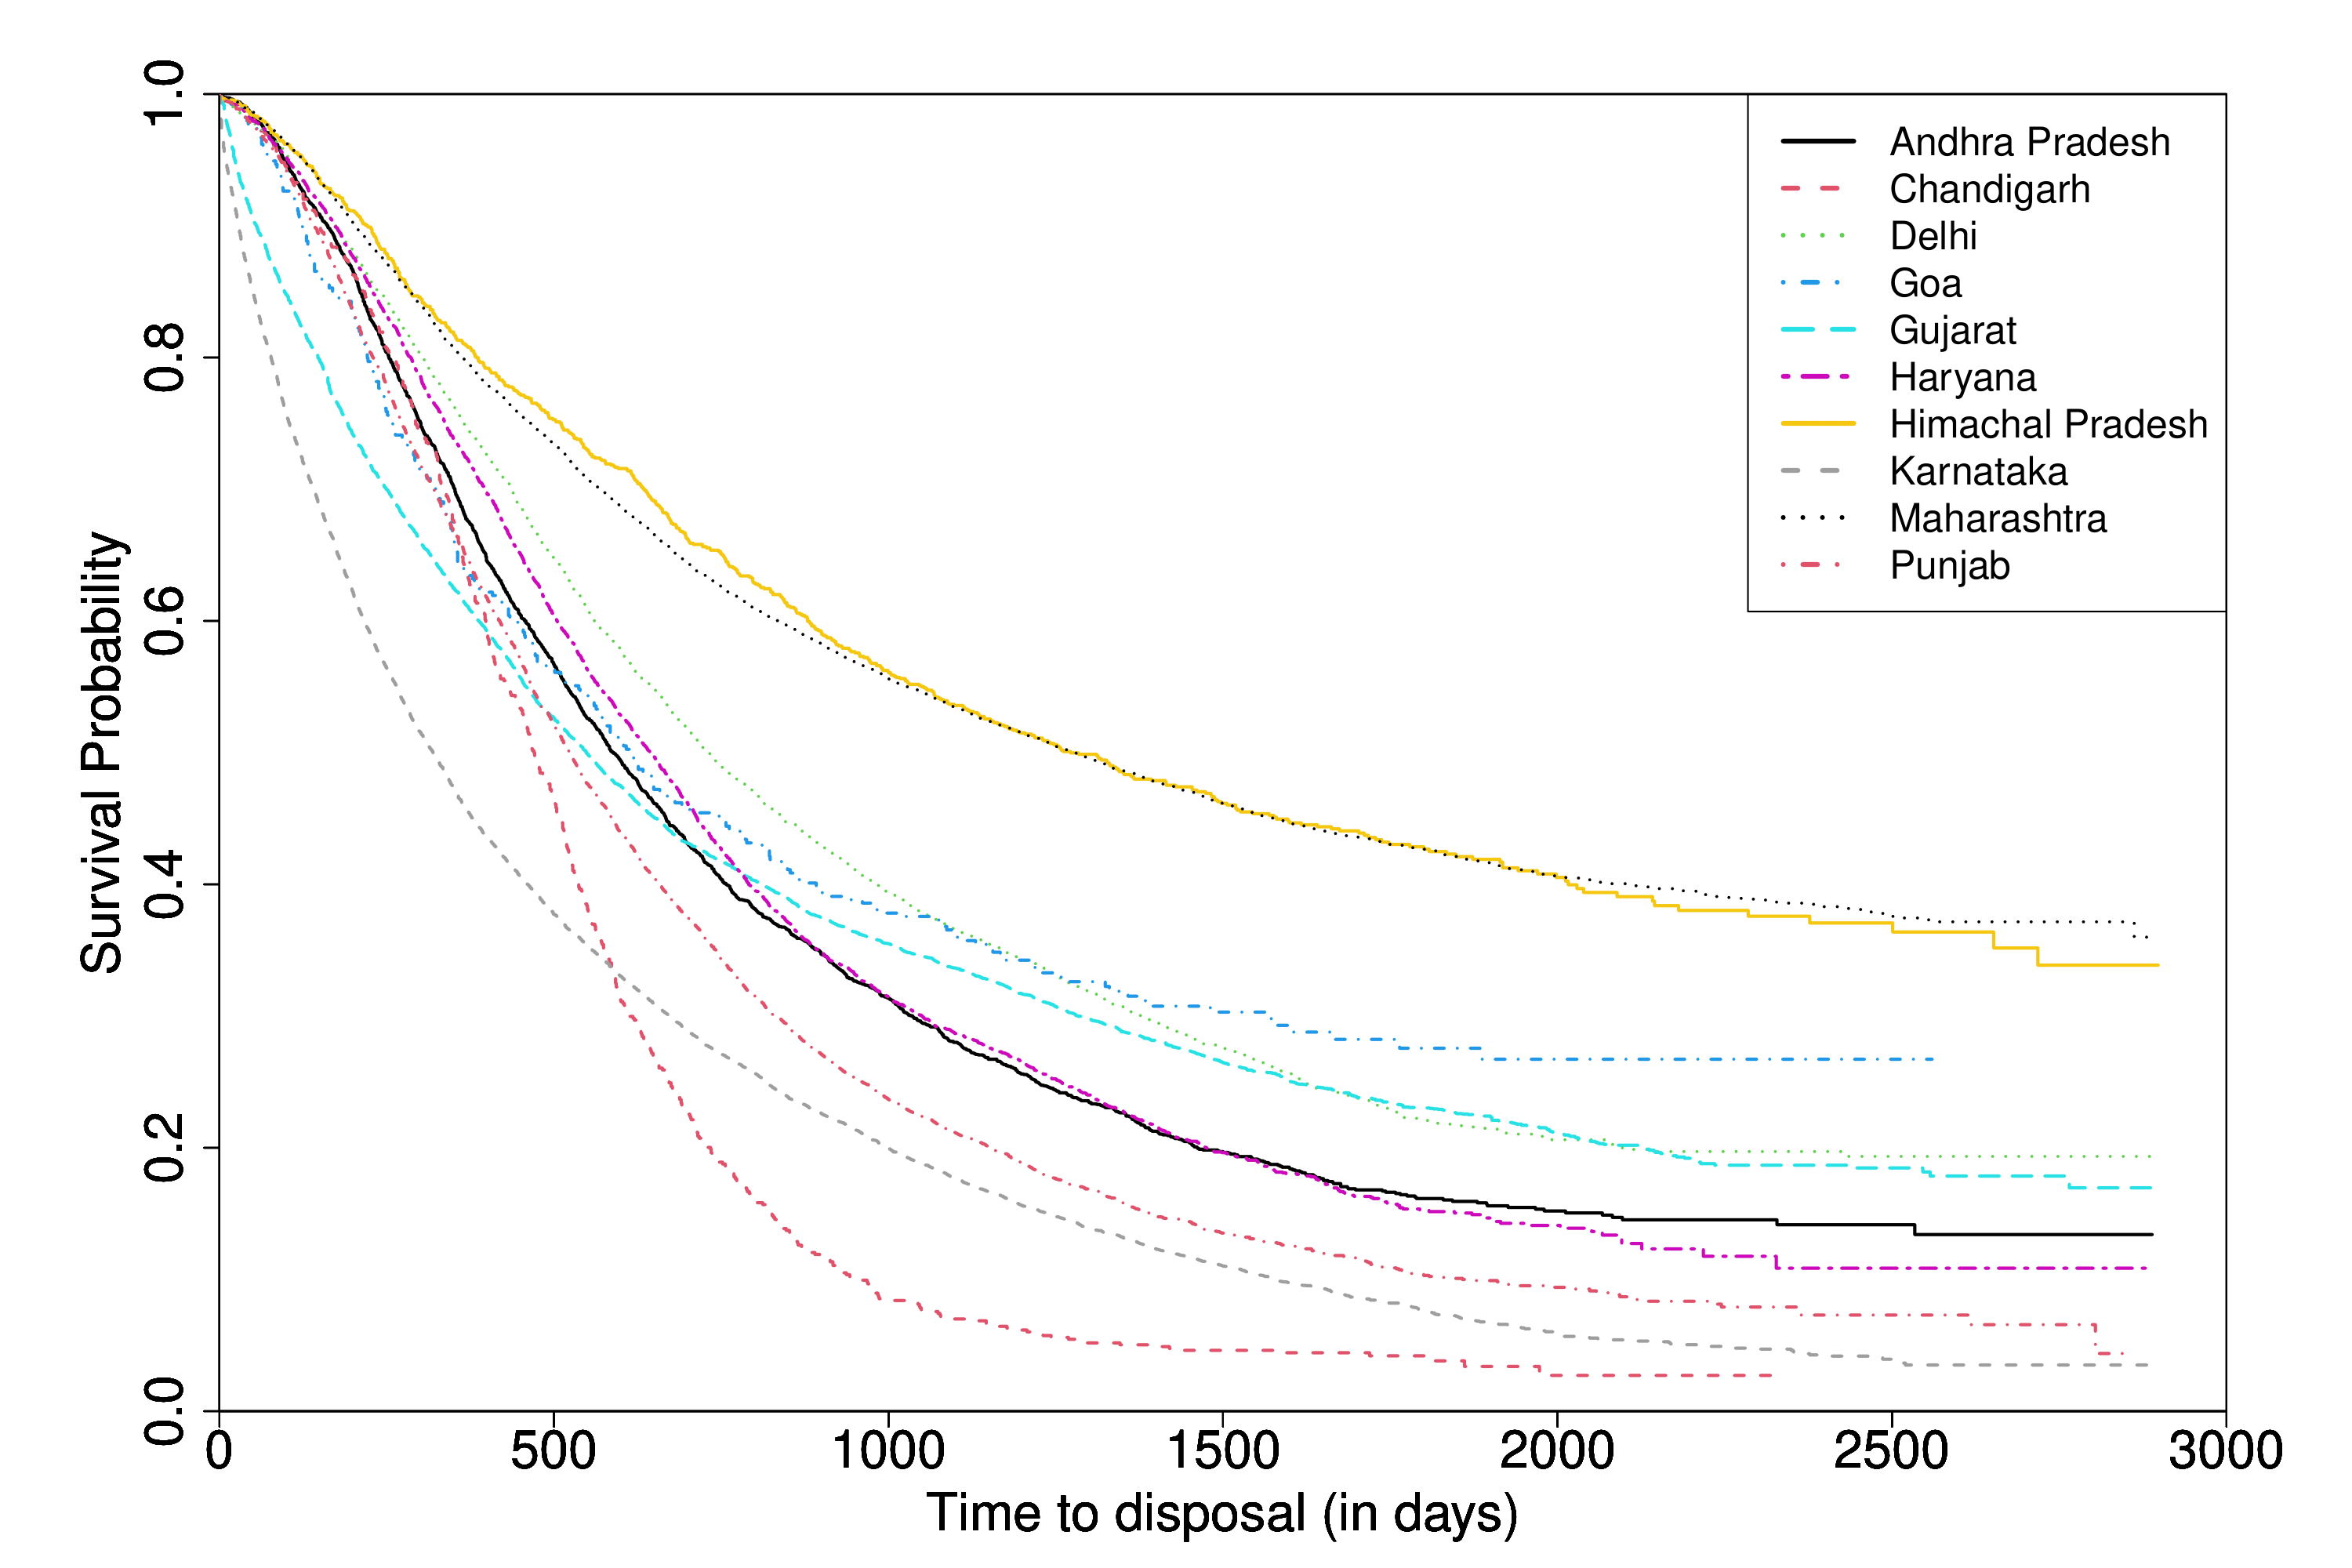
\includegraphics[width = \textwidth]{surv_states-1.png}
\end{figure}

\begin{figure}[h!]
 \centering
 \caption{Survival probability of cases across years}\label{fig:yearSurvival}
 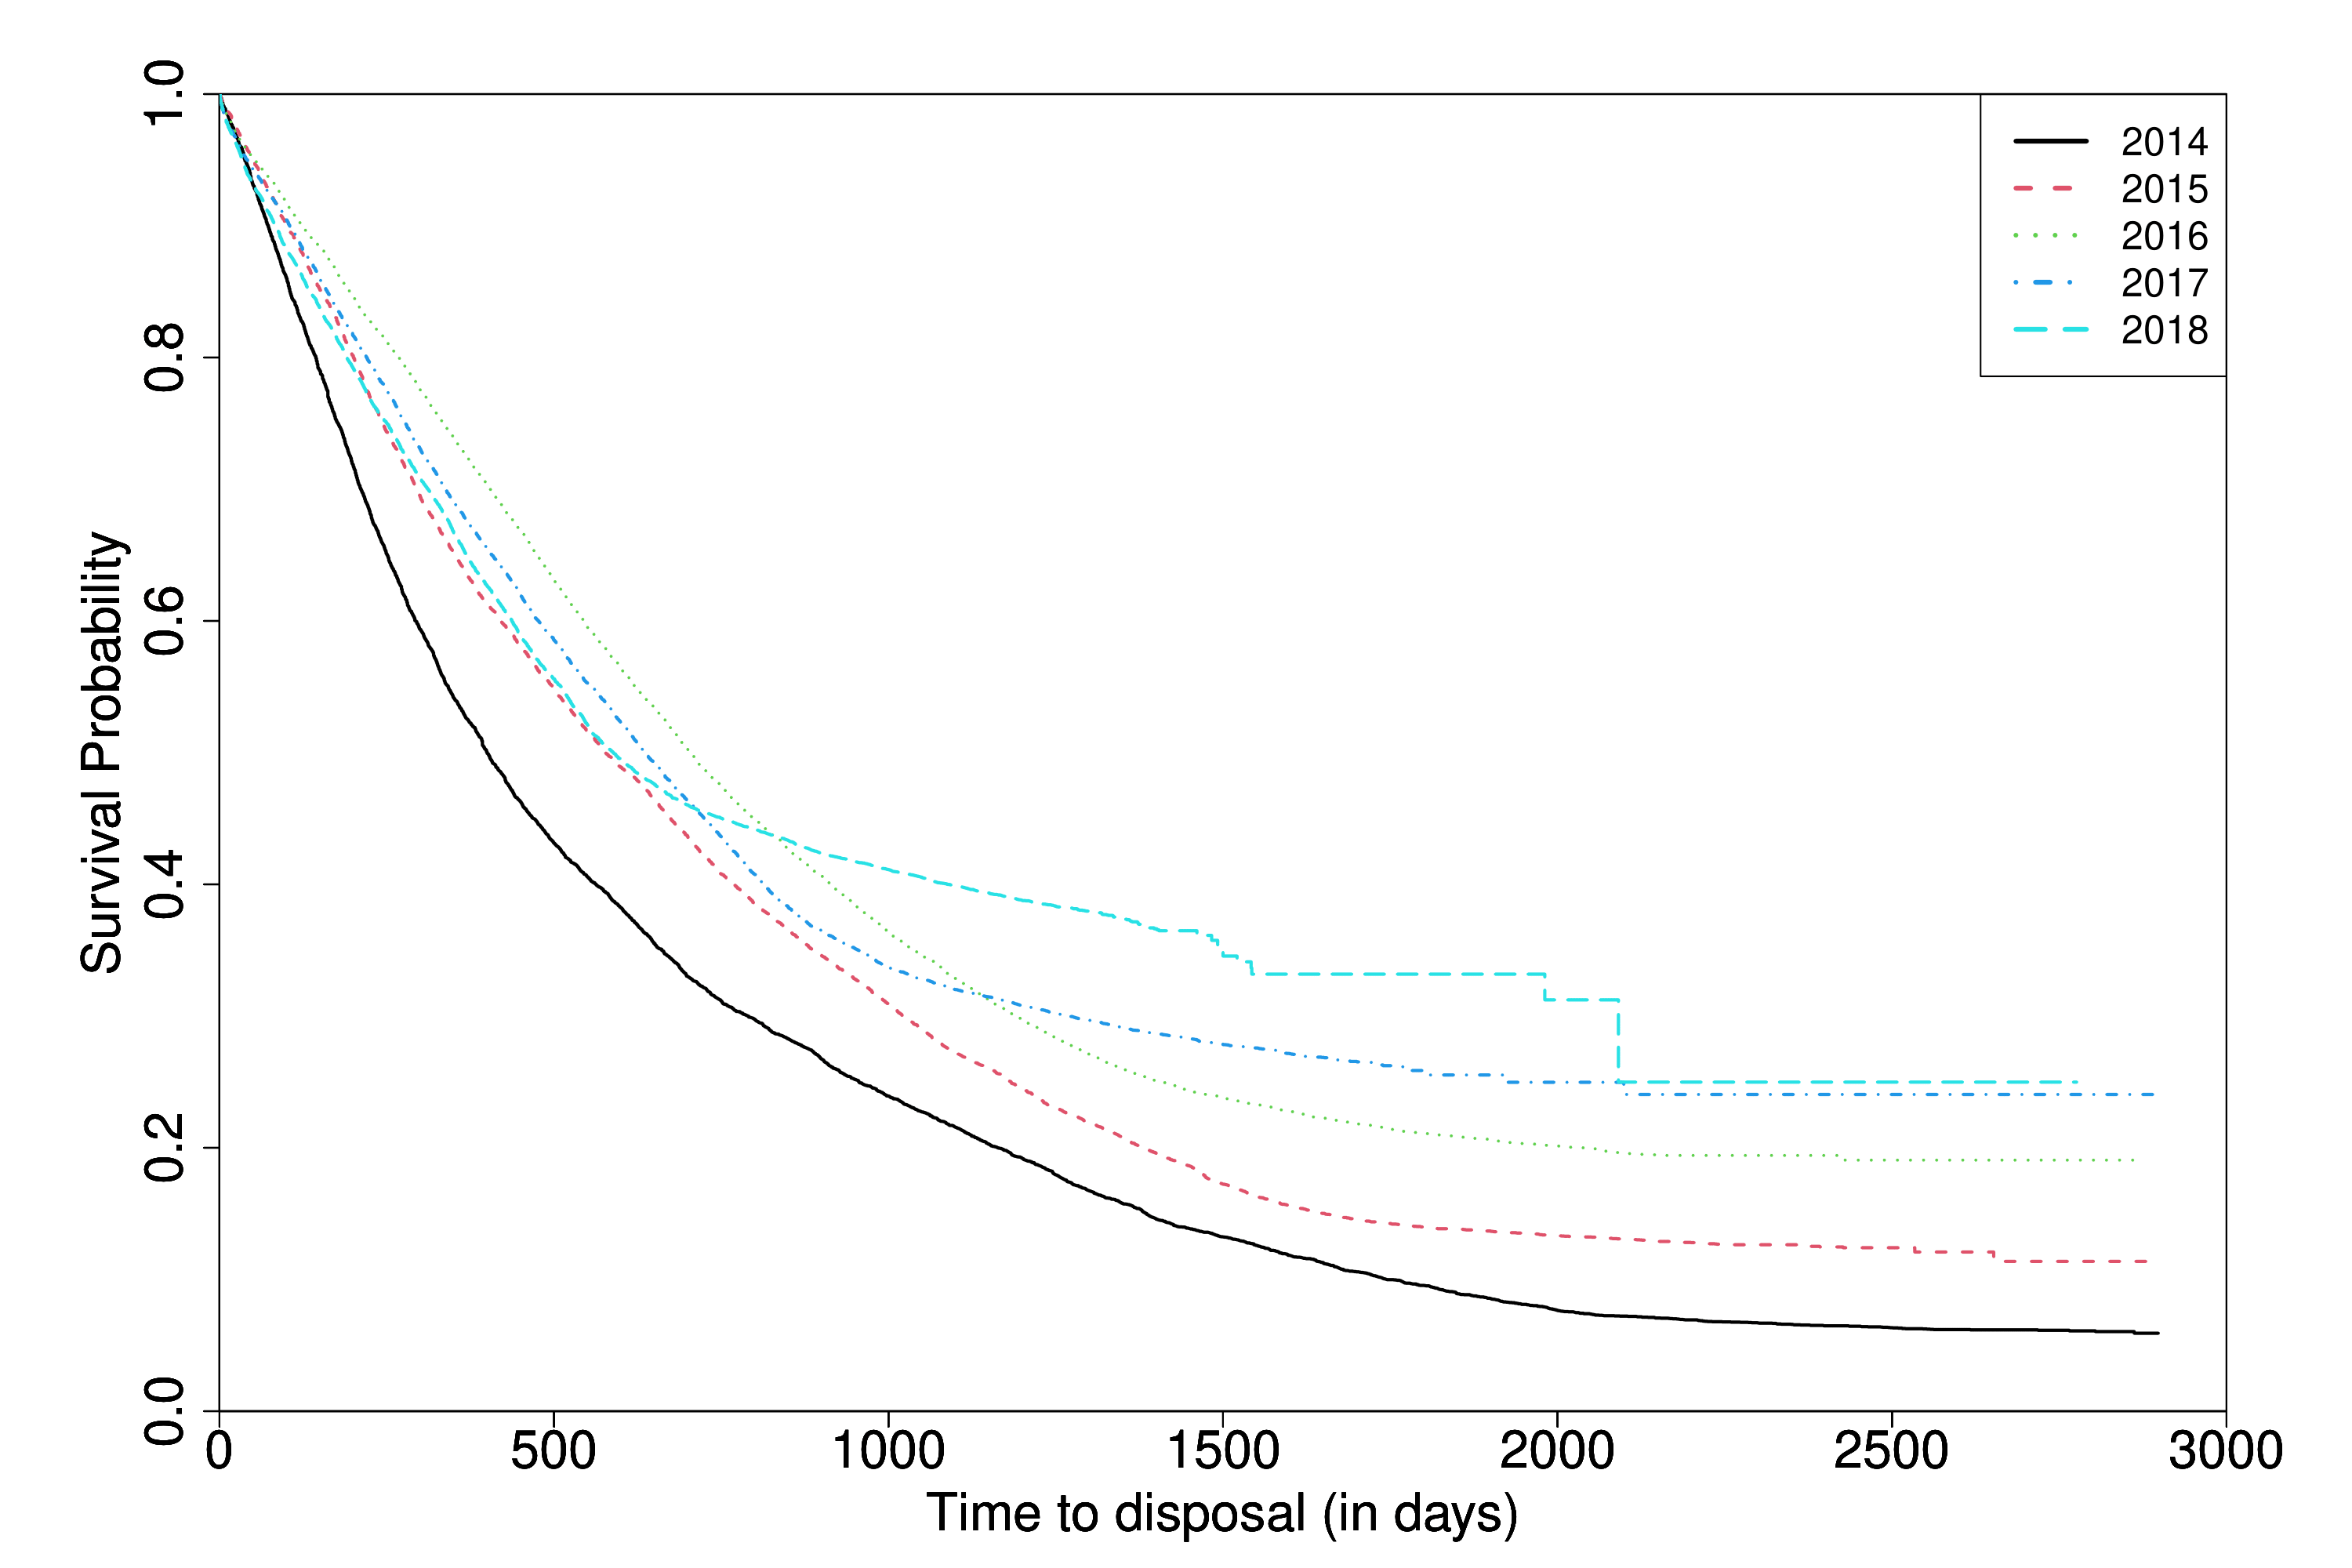
\includegraphics[width = \textwidth]{surv_years-1.png}
\end{figure}

Next we estimate the effect of each case characteristic on the probability of the case getting disposed by the end of the observation period (i.e. 15th September 2021). Like in \textcite{datta2017_itatDelays}, we use the Cox-proportional hazard model to estimate the effect of each case characteristic. Table \ref{tab:survialProb} shows the results of the Cox-proportional hazard model. A negative coefficient indicates a lower probability of the case completing before the end of the observation period, and a positive coefficient indicates a higher probability of the case completing. As an example, jurisdictional issues and non-appearance of the accused reduce the probability of the case concluding (before 15th September 2021) by approximately 71\%, whereas the case being contested increases this probability by 55\%.

\begin{table}[!ht]
  \caption{Regression result: Probability of case completion}\label{tab:survialProb}
  \footnotesize
  \begin{tabular}{lr}
    \\[-1.8ex] 
    \hline \\[-1.8ex] 
    & \multicolumn{1}{c}{\textit{Dependent variable: Probability of case completion}} \\ 
    \cline{2-2} 
    % \\[-1.8ex] & time \\
    \hline \\[-1.8ex] 
			
    D(non-Appearance) & $-$0.712$^{***}$ \\ 
    & (0.013) \\ 
    % & \\
    D(Summons)) & $-$0.286$^{***}$ \\ 
    & (0.015) \\ 
    % & \\
    D(Mediation)) & 0.097$^{***}$ \\ 
    & (0.013) \\ 
    % & \\
    D(Jurisdiction)) & $-$0.716$^{***}$ \\ 
    & (0.013) \\ 
    % & \\
    D(Multiple cheques)) & $-$0.235$^{***}$ \\ 
    & (0.027) \\ 
    % & \\
    D(D(Contested)) & 0.553$^{***}$ \\ 
    & (0.015) \\ 
    \hline \\[-1.8ex]
    State & Y \\
    Year & Y \\ 
    \hline \\[-1.8ex]
    Observations & 46,304 \\ 
    R$^{2}$ & 0.274 \\ 
    Max. Possible R$^{2}$ & 1.000 \\ 
    Log Likelihood & $-$353,508.100 \\ 
    Wald Test & 14,569.790$^{***}$ (df = 19) \\ 
    LR Test & 14,819.270$^{***}$ (df = 19) \\ 
    Score (Logrank) Test & 15,224.080$^{***}$ (df = 19) \\ 
    \hline 
    \hline \\[-1.8ex] 
    \textit{Note:}  & \multicolumn{1}{r}{$^{*}$p$<$0.1; $^{**}$p$<$0.05; $^{***}$p$<$0.01} \\ 
  \end{tabular}
\end{table}

The only result that contradicts the findings of the fixed-effects model is the effect of mediation on case duration. The results of Cox-proportional hazard model indicate that being referred to mediation increases the probability of the case concluding within the observation period by 9.7\%. However, as we have mentioned earlier, we cannot reliably identify case characteristics in pending cases. Therefore, this result has to be interpreted with some caution.

%%% Local Variables:
%%% mode: latex
%%% TeX-master: "paper_chequeDishonour"
%%% End:
\end{appendices}

\newpage
\printbibliography[heading=bibintoc]

\end{document}

%%% Local Variables:
%%% mode: latex
%%% TeX-master: t
%%% End: